\section{ОСНОВНЫЕ ПОНЯТИЯ И МЕТОДЫ ЛИНЕЙНОГО ПРОГРАММИРОВАНИЯ}

В 1939 году Леонид Витальевич Канторович опубликовал работу «Математические методы организации и планирования производства», в которой сформулировал новый класс экстремальных задач с ограничениями и разработал эффективный метод их решения. Тем самым были заложены основы линейного программирования. Джордж Данциг разработал симплекс метод и считается «отцом линейного программирования» на западе. Слово программирование здесь означает составление оптимального плана (программы) производства.

\subsection{Формулировка задач линейного программирования. Основные формы линейных моделей}

Сущность линейного программирования состоит в нахождении точек наибольшего или наименьшего значения некоторой линейной функции при определенном наборе линейных ограничений, налагаемых на аргументы. Ограничения образуют \textit{систему ограничений}, которая имеет, как правило, бесконечное множество решений. Каждая совокупность значений переменных (аргументов функции $z$), которые удовлетворяют системе ограничений, называется \textit{допустимым планом} задачи линейного программирования. Функция $z$, максимум или минимум которой определяется, называется \textit{целевой функцией задачи}. Допустимый план, на котором достигается  максимум или минимум функции $z$, называется \textit{оптимальным планом задачи.} Система ограничений, определяющая множество планов, диктуется условиями производства. Задача линейного программирования состоит в выборе из множества допустимых планов наиболее выгодного (оптимального).

\primer{Мастерская имеет два станка $S_1$, $S_2$ на которых последовательно обрабатывается два вида продукции $P_1$ и  $P_2$. Станок $S_1$ обрабатывает единицу продукции  $P_1$ за 1 час, а единицу продукции  $P_2$ — за 2 часа. Станок  $S_2$ затрачивает на единицу продукции $P_1$  2 часа, а на единицу продукции $P_2$ — 1 час. Станок $S_1$ может работать в сутки не более 10 часов, а станок $S_2$ — не более 8 часов. Стоимость единицы продукции $P_1$ составляет c 1 рублей, а стоимость единицы продукции $P_2$ — c 2 рублей. Требуется определить такой суточный план выпуска двух видов продукции $P_1$ и $P_2$ мастерской, чтобы выручка от реализации произведенной продукции была максимальна.}

Обозначим через $x_1$ и $x_2$ количество продукции $P_1$ и $P_2$ соответственно, которые планируется произвести на станках $S_1$ и $S_2$. Стоимость произведенной продукции  \( z = c_1x_1 + c_2x_2\). Мы должны назначить $x_1$ и $x_2$ так, чтобы величина $z$ была максимальной. Переменные $x_1$ и $x_2$ не могут принимать произвольных значений. Их значения ограничены условиями производства, а именно, тем, что станки могут работать ограниченное время. На изготовление продукции $P_1$ станок $S_1$  тратит $1\cdot x_1$ часов, а на изготовление продукции $P_2$  — $2\cdot x_2$ часов. Поскольку время работы станка $S_1$ не превосходит 10 часов, то величины $x_1$ и $x_2$ должны удовлетворять неравенству \(x_1 + 2\cdot x \leq 10\). Аналогично можно получить неравенство для станка $S_2$: \(2\cdot x_1 + x_2 \leq 8\) . Кроме того, величины $x_1$ и $x_2$ не могут быть отрицательными: $x_1$0, $x_2$0.

Таким образом, задача заключается в нахождении точек максимума функции $z$ среди точек с координатами $x_1$ и $x_2$, которые удовлетворяют указанным неравенствам. Такие задачи кратко записываются следующим образом:

\[z=c_1 x_1 + c_2 x_2 \rightarrow max\]
$$
\left\{
\begin{array}{ll}
x_1+2x_2\leq 10, \\
2x_2+x_1\leq 8; \\
\end{array}
\right.
$$
\[x_1\geq 0; x_2\geq 0.\]


Рассмотрим несколько экономико-математических моделей, допускающих формулировки в виде задач линейного программирования.

\textit{Задача об оптимальном составе смеси.} Эта задача является одной из первых задач, решенных методами линейного программирования. Изложим ее как задачу определения оптимального рациона кормления скота. Пусть нам известно содержание необходимых для кормления животного питательных веществ в различных применяемых кормах. Известна также стоимость единицы каждого вида корма. Требуется составить рацион — набор и количество кормов — так, чтобы каждое питательное вещество содержалось в нем в необходимом количестве и чтобы суммарные расходы на этот рацион были минимальны. Введем следующие обозначения:

$m$ — число различных питательных веществ (витаминов, белков, углеводов и т. д.);

$n$ — число применяемых видов кормов (силос, сено и т. д.);

$a_{ik}$ — количество единиц $i$-го питательного вещества, содержащегося в единице $k$-го вида кормов;

$b_i$ — минимальная суточная потребность животного в $i$-ом питательном веществе;

$c_k$  — стоимость единицы $k$-го вида корма;

$x_k$  — количество единиц $k$-го вида корма, используемое в суточном рационе и подлежащее определению.

Оптимальным планом здесь являются такие числа $x_1$, $x_2$,\ldots, $x_n$ которые удовлетворяют следующим ограничениям:

\(x_1 \geq 0 , x_2 \geq 0 , \dots , x_n \geq 0 \) (количество корма не может быть отрицательным),

\(\sum\limits_{k=1}^n a_{ik} x_k \geq b_i ,\: i=1,2, \dots, m\) (общее количество $i$-го питательного вещества в рационе не может быть ниже заданного $b_i$), и минимизируют суммарную стоимость составляемого рациона
$$
z=\sum\limits_{k=1}^n c_k x_k \rightarrow \min
$$

Отметим, что такая же математическая задача возникает при отыскании оптимального \textit{состава шихты} в металлургическом производстве. Известно, что для получения легированной стали нужно использовать шихту определенного химического состава. В состав шихты входят весьма дорогостоящие ингредиенты. В то же время можно использовать и малоценные материалы (чугун, лом, отходы с определенным содержанием присадок). Возникает задача отыскания такого состава шихты, который содержал бы необходимые количества химических веществ и имел бы минимальную стоимость. Математическая модель этой задачи совпадает с сформулированной выше. Еще один пример возникновения такой модели дает задача об оптимальном \textit{смешивании нефтепродуктов}. Бензины разных сортов получают путем смешивания нефтепродуктов, имеющих различные технические характеристики. Заданные показатели качества бензина должны выдерживаться весьма точно. С другой стороны, от того, какие нефтепродукты смешиваются и в каком количестве, зависит рентабельность производства. Требуется построить такой план смешивания, который обеспечивал бы максимальную рентабельность производства и позволял, в то же время, получать бензины заданных сортов.

\textit{Задача об оптимальном использовании ресурсов}. Эта задача возникает при составлении планов выпуска продукции предприятием и имеет важное практическое значение. Пусть номенклатура выпускаемой продукции состоит из $n$ наименований. Производство продукции использует $m$ видов ресурсов. Обозначим через $a_{ik}$ затраты $i$-го вида ресурсов $(i= 1, 2,\, \dots\, , m)$ на производство единицы продукции $k$-го вида $(k = 1, 2,\, \dots\, , n)$. Пусть $b_i$ — полный объем ресурсов $i$-го вида $(i = 1, 2,\, \dots\, , m)$, а $c_k$  — прибыль, получаемая предприятием при изготовлении и реализации единицы $k$-го вида продукции $(k = 1, 2,\, \dots\, , n)$. Требуется составить такой план выпуска продукции, который был бы технологически осуществим по имеющимся ресурсам и, в то же время, приносил наибольшую общую прибыль предприятию. Математическая модель задачи состоит в следующем. Обозначим  через \(X = \left\{ x_1, x_2,\, \dots \, , x_n \right\}\) номенклатурный план выпуска продукции. Величины $x_k$ должны удовлетворять следующим условиям:

\(x_1 \geq 0 , x_2 \geq 0 , \dots , x_n \geq 0 \) (количество производимой продукции не может быть отрицательным),

\(\sum\limits_{k=1}^n a_{ik} x_k \geq b_i ,\: i=1,2, \dots, m\) (технологические ограничения).
Кроме того, общая прибыль от производства и реализации продукции должна быть максимальной.
$$
z=\sum\limits_{k=1}^n c_k x_k \rightarrow \max
$$

Приведение примеров математических моделей задач планирования и управления можно продолжить. Ниже мы еще вернемся к некоторым из таких моделей. Сейчас обсудим форму возникающих задач независимо от их содержания. Все задачи были задачами на минимум или максимум линейной целевой функции с ограничениями неравенствами. Переменные подчинялись условиям неотрицательности.

В других ситуациях могут возникать задачи, в систему ограничений которых, кроме неравенств, могут входить и равенства. Поэтому в наиболее общей форме задачу линейного программирования формулируют следующим образом:


\[z=c_0+c_1x_1+c_2x_2+\dots+c_nx_n \rightarrow \max (\min)\]
$$
\left\{
\begin{array}{ll}
	a_{11}x_1+a_{12}x_2+\dots+a_{1n}x_n \, R_1 b_1 \\
	a_{21}x_1+a_{22}x_2+\dots+a_{2n}x_n \, R_2 b_2 \\
	\dots\dots\dots\dots\dots\dots\dots\dots\dots\dots\dots\\
	a_{m1}x_1+a_{m2}x_2+\dots+a_{mn}x_n \, R_m b_m \\
\end{array}
\right.
$$

где $R_j (j=1, 2,\,\dots\,, m)$— один из знаков сравнения $(\leq, \geq, = )$.

Одна и та же задача линейного программирования может быть сформулирована в различных эквивалентных формах. Наиболее важными формами задачи линейного программирования являются \textit{каноническая и стандартная}.
В \textit{канонической форме} задача является задачей на максимум некоторой линейной функции $z$, а ее система ограничений состоит только из равенств (уравнений); при этом переменные задачи $x_1, x_2, \,\dots\, x_n$ являются неотрицательными:

\[z=c_0+c_1x_1+c_2x_2+\dots+c_nx_n \rightarrow \max \]
$$
\left\{
\begin{array}{ll}
	a_{11}x_1+a_{12}x_2+\dots+a_{1n}x_n \,= b_1 \\
	a_{21}x_1+a_{22}x_2+\dots+a_{2n}x_n \,= b_2 \\
	\dots\dots\dots\dots\dots\dots\dots\dots\dots\dots\dots\\
	a_{m1}x_1+a_{m2}x_2+\dots+a_{mn}x_n \,= b_m \\
\end{array}
\right.
$$
\[x_1\geq 0, x_2 \geq 0, \dots, x_n \geq 0.\]

К канонической форме можно привести любую задачу линейного программирования. Если в исходной задаче некоторое ограничение (например, первое) было неравенством, то оно преобразуется в равенство введением в левую часть некоторой неотрицательной переменной. Действительно

$$
a_{11}x_1+a_{12}x_2+\,\dots\,+a_{1n}x_n\leq b_1.
$$

Вводим переменную  \(x_{n+1}=b_1-a_{11}x_1-a_{12}x_2-\dots-a_{1n}x_n.\) Тогда неравенство запишется в виде

$$
a_{11}x_1+a_{12}x_2+\dots+a_{1n}x_n+x_{n+1}=b_1
$$

В каждое из неравенств вводится своя “уравнивающая” переменная, после чего система ограничений становится системой уравнений. При этом “уравнивающая” переменная автоматически будет неотрицательной. Если в исходной задаче некоторая переменная $x_i$ не подчинена условию неотрицательности, то ее заменяют разностью неотрицательных переменных $x'_i$ и $x''_i$ :

$$
x_i=x''_i-x'_i;\, x'_i, x''_i \leq 0.
$$

Наконец, если исходная задача была задачей на минимум, то введением новой целевой функции $z_1=-z$ мы преобразуем нашу задачу на минимум функции $z$ в задачу на максимум функции $z_1$.

Таким образом, всякую задачу линейного программирования можно сформулировать в канонической форме.

В \textit{стандартной форме} задача линейного программирования является задачей на максимум линейной целевой функции. Система ограничений ее состоит из линейных неравенств типа «$\geq$». Все переменные задачи неотрицательны.

\[z=c_0+c_1x_1+c_2x_2+\dots+c_nx_n \rightarrow \max (\min)\]
$$
\left\{
\begin{array}{ll}
	a_{11}x_1+a_{12}x_2+\dots+a_{1n}x_n \, b_1 \\
	a_{21}x_1+a_{22}x_2+\dots+a_{2n}x_n \, b_2 \\
	\dots\dots\dots\dots\dots\dots\dots\dots\dots\dots\dots\\
	a_{m1}x_1+a_{m2}x_2+\dots+a_{mn}x_n \,  b_m \\
\end{array}
\right.
$$
\[x_1 \leq 0, x_2 \leq 0, \,\dots\, ,x_n \leq 0. \]

Всякую задачу линейного программирования можно сформулировать в стандартной форме. Преобразование задачи на минимум в задачу на максимум, а также обеспечение неотрицательности переменных производится, как и раньше. Всякое равенство в системе ограничений равносильно системе взаимно противоположных неравенств:

$$
a_{i1}x_i+a_{i2}x_2+\dots+a_{in}x_n=b_i	\leftrightarrow
\left\{
\begin{array}{ll}
	a_{i1}x_i + a_{i2}x_2 + \dots + a_{in}x_n \leq b_i\\
	- a_{i1}x_i - a_{i2}x_2 - \dots - a_{in}x_n \leq - b_i\\
\end{array}
\right.
$$

Существуют и другие способы преобразования системы равенств в систему неравенств, то есть всякую задачу линейного программирования можно сформулировать в стандартной форме.

Рассмотренные выше записи задач линейного программирования в канонической и стандартной формах обычно называют скалярными записями. Иногда более удобной является векторно-матричная запись. Введем векторы
$$
\vec x=\{x_1, x_2, \dots, x_n \}, \;\; \vec c=\{c_1, c_2, \dots, c_n \}, \;\; \vec b=\{b_1, b_2, \dots, b_n \}
$$
и матрицу $A=(a_{ij})$ коэффициентов в системе ограничений. Тогда задачи в канонической и стандартной формах можно записать соответственно в виде

$$
\begin{array}{ll}
z = c_0 + (\vec c, \vec x) \rightarrow \max, \\
A\vec x= \vec b, \vec x \geq \vec 0 \\
\end{array}
$$

$$
\begin{array}{ll}
z = c_0 + (\vec c, \vec x) \rightarrow \max, \\
A\vec x\leq \vec b, \vec x \geq \vec 0 \\
\end{array}
$$

Здесь и ниже неравенство $\vec a \leq \vec e \;(\vec a < \vec e)$ между векторами одинаковой размерности означает, что выполнены неравенства между всеми соответствующими координатами этих векторов. При этом условия неотрицательности (положительности) переменных часто записывают просто в виде $\vec x \geq 0 \; (\vec x > 0)$.

В заключение параграфа отметим, что произвольная задача линейного программирования может не иметь решения. Эта ситуация может возникнуть в двух случаях: 1) система ограничений несовместна (область допустимых планов пуста); 2) целевая функция задачи неограничена на области допустимых планов. В первом случае задачу называют \textit{недопустимой}.

\subsection{Геометрическое истолкование задачи в стандартной форме в случае двух переменных}

Задача линейного программирования в стандартной форме с двумя перемененными имеет вид:

\begin{gather*}
z = c_{0} + c_{1}x_{1} + c_{2}x_{2} \rightarrow max;\\
\begin{cases}
a_{11}x_{1} + a_{12}x_{2} \le b_{1},\\
a_{21}x_{1} + a_{22}x_{2} \le b_{2},\\
...............................\\
a_{m1}x_{1} + a_{m2}x_{2} \le b_{m};
\end{cases}\\
x_{1},x_{2} \ge 0.
\end{gather*}

Эти задачи допускают простое геометрическое истолкование. Рассмотрим вначале геометрическое истолкование системы ограничений задачи. Каждую совокупность значений переменных $x1, x2$ можно изобразить точкой на плоскости, если ввести систему координат и по одной оси откладывать $x1$, а по другой — $x2$. Выясним, что геометрически означает совокупность решений одного отдельно взятого неравенства

$$a_{1}x_{1} + a_{2}x_{2} \le b.$$
\\Рассмотрим прямую линию на плоскости с уравнением

$$a_{1}x_{1} + a_{2}x_{2} = b.$$

Эта прямая делит плоскость на две полуплоскости, в одной из которых справедливо наше неравенство, а в другой — противоположное неравенство. Чтобы проверить, какая из полуплоскостей состоит из решений нашего неравенства, следует взять точку из какой-либо полуплоскости и проверить, выполняется ли наше неравенство в этой точке. Множество решений отдельно взятого линейного неравенства представляет собой полуплоскость. Для системы из нескольких таких неравенств точки, координаты которых удовлетворяют всем неравенствам одновременно, должны находиться во всех соответствующих полуплоскостях, то есть  принадлежать теоретико-множественному пересечению этих  полуплоскостей. Множество точек на плоскости, удовлетворяющих системе ограничений, составляет, таким образом, некоторую выпуклую многоугольную область. Условия неотрицательности переменных
$x1, x2 \ge0$ приводят к тому, что эта область находится в первой координатной четверти.

\primer{Построим на плоскости множество решений системы неравенств (рис.1.1)}

$$\begin{cases}
x_{1} + 2x_{2} \le 10,\\
2x_{1} + x_{2} \le 8
\end{cases}\\
\hspace{36mm}
x_{1} \ge 0; x_{2} \ge 0.$$

\begin{figure}
  \centering
  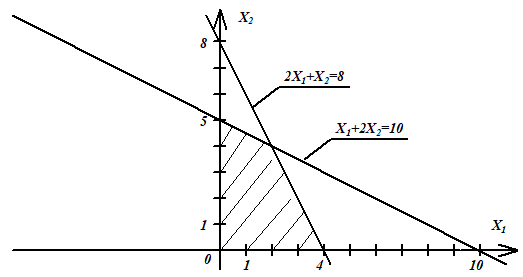
\includegraphics[width=0.7\linewidth]{pictures/picturefile_1_1}
  \caption{}
  \label{fig:grafic1}
\end{figure}

Множество точек на плоскости, удовлетворяющих системе ограничений задачи, называют часто допустимым многоугольником. Эта область может быть неограниченной или вовсе пустой.

Целевая функция задачи геометрически изображается с помощью прямой уровня, то есть прямой, на которой\\
$$z = c_{0}+c_{1}x_{1} + c_{2}x_{2}$$
принимает постоянное значение. Если C — произвольная константа, то уравнение прямой уровня имеет вид $c_{0}+c_{1}x_{1} + c_{2}x_{2} = C$

При изменении константы $C$ мы получаем различные прямые, параллельные друг другу. При увеличении C прямая уровня перемещается в направлении наискорейшего возрастания функции $z$, то есть, в направлении ее градиента. Вектор градиента\\
$$grad z = \left\{\frac{\delta z}{\delta x_{1}};\frac{\delta z}{\delta x_{2}}\right\} = \left\{c_{1},c_{2}\right\}$$

Геометрический метод решения задачи состоит в следующем. Строится допустимый многоугольник и некоторое положение линии уровня целевой функции. Определяется направление перемещения прямой уровня. Точкой минимума $z$  будет точка первого касания линии уровня с допустимым многоугольником. Точкой максимума — точка отрыва линии уровня от допустимого многоугольника. Эти  точки чаще всего совпадают с некоторыми вершинами допустимого  многоугольника. Таких точек может быть бесчисленное множество, если линия уровня $z$ параллельна одной из сторон допустимого многоугольника.

\primer{Решим геометрически задачу примера 1.1 при $c_{1} = 1, c_{2} = 1$ (рис 1.2).}

\begin{figure}
\centering
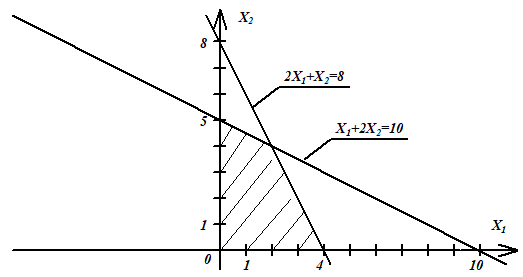
\includegraphics[width=0.7\linewidth]{pictures/picturefile_1_1}
\caption{}
\label{fig:grafic2}
\end{figure}

Точкой максимума  здесь является точка A, координаты которой определяются из следующей системы уравнений:\\

$$\begin{cases}
x_{1} + 2x_{2} =10,\\
2x_{1} + x_{2} =8.
\end{cases}$$\\
Решая эту систему, получаем  точку максимума $A(2,4), z_{max} =6$.

\subsection{Общие системы линейных уравнений. Базисный вид системы. Метод Гаусса-Жордана}
Ниже нам понадобятся некоторые сведения о системах уравнений, состоящих из m линейных уравнений с \textit {n} неизвестными $x_1$,$x_2$,\dots,$x_\textit{n}$

\begin{equation*}
\begin{cases}
a_{11}x_1 + a_{12}x_1 + \dots + a_{1n}x_1 =b_1\\
a_{21}x_1 + a_{22}x_1 + \dots + a_{2n}x_1 =b_2\\
\dots\dots\dots\dots\dots\dots\dots\dots\dots\dots\dots\\
a_{m1}x_1 + a_{m2}x_1 + \dots + a_{mn}x_1 =b_m
\end{cases}
\end{equation*}

Такая система может иметь множество решений, состоящее из единственного решения или бесконечного количества решений. Возможен также случай \textit{несовместности системы}, когда множество решений является пустым. Две системы называются\textit {эквивалентными}, если они имеют одинаковые множества решений. Следующие операции над системой приводят к новой системе, эквивалентной исходной:
		\begin{enumerate}
			\renewcommand{\theenumi}{(\arabic{enumi})}
			\renewcommand{\labelenumi}{\arabic{enumi})}
			\itemперестановка уравнений системы;
			\itemумножение обеих частей уравнения системы на одно и то же отличное от нуля число;
			\itemприбавление к заданному уравнению системы любого другого уравнения, умноженного на произвольное число.
		\end{enumerate}
Эти операции называют элементарными операциями над системой.

Основной задачей теории линейных систем является задача нахождения всего множества решений системы или установления ее несовместности. Для ее решения нужно привести систему к эквивалентной системе, имеющей особый \textit{базисный вид}. При этом систему условно записывают в виде расширенной матрицы системы

$$\left(\begin{array}{rrrr|r}
a_{11}&a_{12}&\dots&a_{1n}&b_1\\
a_{21}&a_{22}&\dots&a_{2n}&b_2\\
\dots&\dots&\dots&\dots&\dots\\
a_{m1}&a_{m2}&\dots&a_{mn}&b_m\\
\end{array}\right)$$

Система называется имеющей базисный вид, если среди столбцов коэффициентов при неизвестных в ее расширенной матрице имеется столько  различных  единичных  столбцов, сколько  ненулевых строк в этой матрице. Единичным столбцом мы называем столбец, в котором на некотором месте стоит единица, а на всех остальных местах — нули. Единичные столбцы считаются различными, если единицы у них находятся на различных местах. Неизвестные, отвечающие этим различным единичным столбцам, называются \textit{базисными неизвестными системы}. Остальные неизвестные называются \textit{свободными неизвестными}. Базисные неизвестные входят по одному в каждое из уравнений и легко выражаются через свободные неизвестные. Если свободным неизвестным придавать произвольные значения, то базисные неизвестные по ним определятся однозначно, и мы получим все решения системы.

\primer{Рассмотрим систему
\begin{equation*}
\begin{cases}
x_1+ 3x_2+ 5x_3 = 6,\\
7x_2- 2x_3+ x_4 = -1.\\
\end{cases}
\end{equation*}

Ее расширенная матрица
$$\left(\begin{array}{rrrr|r}
1&3&5&0&6\\
0&7&-2&1&-1\\
\end{array}\right).$$

Система имеет базисный вид. Базисными неизвестными будут $x_1$ и $x_4$, а свободными — $x_2$ и $x_3$.
\begin{equation*}
\begin{cases}
x_1 = 6-3x_2 -5x_3\\
x_4 = -1 -7x_2 +2x_3.\\
\end{cases}
\end{equation*}

Полагая, свободные неизвестные произвольными $x_2=c_1$, $x_3=c_2$, получаем двухпараметрическое семейство всех решений нашей системы ($6-3c_1-5c_2;c_1;c_2;-1-7c_1+2c_2$).}

Свободные неизвестные могут отсутствовать в базисном виде системы. Тогда, очевидно, система имеет только одно решение.

Метод Гаусса-Жордана представляет собой некоторый алгоритм, приводящий систему к базисному виду с помощью цепочки элементарных преобразований, которую удобно выполнять не над системой, а над ее расширенной матрицей. При этом элементарные операции над системой становятся следующими операциями над расширенной матрицей:
		\begin{enumerate}
			\renewcommand{\theenumi}{(\arabic{enumi})}
			\renewcommand{\labelenumi}{\arabic{enumi})}
			\itemперестановка строк в матрице;
			\itemумножение всех элементов некоторой строки на одно и то же отличное от нуля число;
			\itemприбавление к данной строке любой другой, умноженной на произвольное число.
		\end{enumerate}

Метод Гаусса-Жордана состоит из ряда однотипных шагов. Опишем первый шаг алгоритма. Он состоит из трех этапов:
		\begin{enumerate}
			\renewcommand{\theenumi}{(\arabic{enumi})}
			\renewcommand{\labelenumi}{\arabic{enumi})}
			\itemсреди коэффициентов при неизвестных расширенной матрицы системы выбирается отличное от нуля число, которое в дальнейшем мы называем  \textit{разрешающим элементом} шага метода;
			\itemстрока разрешающего элемента делится на разрешающий элемент и полученная строка, становясь основным инструментом для преобразования матрицы, называется нами в дальнейшем \textit{ведущей строкой} шага алгоритма;
			\itemведущая строка преобразует остальные строки матрицы путем прибавления ее к этим строкам после умножения на так подобранные числа, чтобы после преобразований в столбце бывшего разрешающего элемента стояли нули на всех местах, кроме места самого разрешающего элемента (на котором находится единица).
		\end{enumerate}

Описанные преобразования являются цепочкой элементарных операций над расширенной матрицей системы, и после завершения шага алгоритма метода Гаусса-Жордана в матрице появляется единичный столбец. Затем шаги повторяются, но на очередном шаге запрещается выбирать разрешающий элемент в строках, в которых он уже выбирался на предыдущих шагах. Шаги продолжаются до тех пор, пока количество единичных столбцов не сравняется с количеством ненулевых строк расширенной матрицы. Мы получаем систему в базисном виде.

При работе методом Гаусса-Жордана возможны следующие две особые ситуации. В результате выполнения очередного шага могут появиться либо нулевая строка
$(0, 0,\dots, 0|0)$, либо строка вида $(0, 0,\dots, 0|b)$, где $b \neq 0$ . В первом случае в новой системе будет уравнение вида $0*x_1 + 0*x_2 + \dots + 0*x_n=0$, которое является тождеством, справедливым при любых значениях неизвестных. Отбрасывание этого уравнения не меняет множества решений системы, поэтому обычно нулевая строка отбрасывается, и работа алгоритма продолжается. Во втором случае в новой системе появляется уравнение $0*x_1 + 0*x_2 + \dots + 0*x_n \neq 0$, которое не может выполняться. Это свидетельствует о том, что новая и первоначальная системы несовместны. В этом случае работа алгоритма прекращается.

\primer{Реализуем метод Гаусса-Жордана для системы

\begin{equation*}
\begin{cases}
x_1+ 3x_2+ 5x_3 = 2,\\
3x_1- 2x_+ 16x_3 = -3.\\
\end{cases}
\end{equation*}

В расширенной матрице системы выберем разрешающий элемент в первой строке и первом столбце. Получим сразу ведущую строку. Умножая первую строку на (-3) и прибавляя ко второй, получим
$$\left(\begin{array}{rrr|r}
[1]\!&3&5&2\\
3&-2&16&-3\\
\end{array}\right)
\sim \left(\begin{array}{rrr|r}
1&3&5&2\\
0&-11&1&-9\\
\end{array}\right).$$

Выбирая разрешающий элемент во второй строке и третьем столбце, умножая вторую строку на (-5) и прибавляя к первой, получим
$$\left(\begin{array}{rrr|r}
1&3&5&2\\
0&-11&[1]\!&-9\\
\end{array}\right)
\sim \left(\begin{array}{rrr|r}
1&58&0&47\\
0&-11&1&-9\\
\end{array}\right).$$

Последняя матрица соответствует системе уравнений
\begin{equation*}
\begin{cases}
x_1+ 58x_2 = 47,\\
-11x_2+ x_3 = -9.\\
\end{cases}
\end{equation*}
с базисными неизвестными $x_1$, $x_3$ и свободной неизвестной $x_2$.}

Отметим, что рассмотренный нами метод содержит большую долю произвола при выборе разрешающего элемента. Полученный в результате базисный вид системы тоже определяется неоднозначно. У совместной системы существует некоторая конечная совокупность базисных видов.

Переход от одного базисного вида к другому можно произвести с помощью, так называемой, \textit{операции замещения}. Эта операция переводит заданную базисную неизвестную $x_i$ в разряд свободных, а заданную свободную неизвестную $x_j$ — в базисную. Операция замещения состоит в дополнительном шаге алгоритма Гаусса-Жордана с особым выбором разрешающего элемента. Этот элемент выбирается в строке, содержащей единицу при базисной неизвестной $x_i$ и в столбце, отвечающем свободной неизвестной $x_j$. Выполним операцию замещения в базисном виде системы предыдущего примера, замещая свободной переменной  $x_2$ базисную $x_1$
$$\left(\begin{array}{rrr|r}
1&[58]\!&0&47\\
0&-11&1&-9\\
\end{array}\right)
\sim \left(\begin{array}{rrr|r}
1/58&[1]\!&0&47/58\\
0&-11&1&-9\\
\end{array}\right)
\sim \left(\begin{array}{rrr|r}
1/58&1&0&47/58\\
11/58&0&1&-5/58\\
\end{array}\right).$$
Тем самым получен новый базисный вид системы
\begin{equation*}
\begin{cases}
\frac{1}{58}x_1+  x_2 = \frac{47}{58},\\
\frac{11}{58}x_1+ x_3 = -\frac{5}{58}.\\
\end{cases}
\end{equation*}

В следующем параграфе при изучении симплекс-метода мы встретимся с базисным видом линейной системы уравнений и операцией замещения. При этом неизвестные будут называться переменными.



\subsection{Симплекс-метод}
Этот метод является универсальным, применимым к любой задаче линейного программирования в канонической форме. Система ограничений здесь — система линейных уравнений, в которой количество неизвестных обычно  больше  количества  уравнений. Если  ранг  системы равен $r$, то мы можем выбрать $r$ неизвестных, которые выразим через все остальные неизвестные. Для определенности предположим, что выбраны  первые, идущие подряд, неизвестные $x_1,x_2,\dots,x_r$ . Тогда наша система уравнений может быть записана в виде

\begin{equation*}
\begin{cases}
x_1 = b'_1 - a'_{1,r+1}x_{r+1} - \dots - a'_{1n}x_n,\\
x_2 = b'_2 - a'_{2,r+1}x_{r+1} - \dots - a'_{2n}x_n,\\
\dots\dots\dots\dots\dots\dots\dots\dots\dots\dots\dots\\
x_r = b'_r - a'_{r,r+1}x_{r+1} - \dots - a'_{rn}x_n,
\end{cases}
\end{equation*}

К такому виду можно привести любую совместную систему, например методом Гаусса-Жордана. Правда, не всегда можно выражать через остальные первые $r$ неизвестных (мы это сделали для определенности записи). Однако такие $r$ неизвестных обязательно найдутся. Эти неизвестные (переменные) называются \textit{базисными}. Остальные переменные называются   \textit{свободными}. Придавая определенные значения свободным переменным и вычисляя значения базисных (выраженных через свободные), мы будем получать различные решения нашей системы ограничений. Таким образом, можно получить любое ее решение. Нас будут интересовать особые решения, которые  получаются, когда свободные переменные равны нулю. Такие решения  называются \textit{базисными}. Базисных решений столько же, сколько  различных  базисных видов у данной системы ограничений. Базисное решение называется \textit{допустимым базисным решением} или \textit{опорным решением}, если в нем значения переменных неотрицательны. Если в качестве базисных взяты переменные $x_1$,$x_2$,\dots,$x_r$, то решение \{$b'_1$,$b'_2$,\dots,$b'_r$,0,\dots,0\} будет опорным, если $b'_1 \leq 0$,    $b'_2 \leq 0$, \dots, $b'_r \leq 0$. Симплекс-метод основан на следующей теореме, которая называется \textit{фундаментальной теоремой симплекс-метода}.

\teorema{Среди оптимальных планов задачи линейного программирования в канонической форме обязательно есть опорное решение ее системы ограничений. Если оптимальный план задачи единственен, то он совпадает с некоторым опорным  решением.}

Различных опорных решений системы ограничений конечное число. Поэтому решение задачи в канонической форме можно было бы искать  перебором опорных решений и выбором среди них того решения,  для  которого  значение $z$ самое большое. Но, во-первых, все опорные решения неизвестны, и их нужно находить, а во-вторых, в реальных задачах этих решений очень много, и прямой перебор вряд ли возможен. Симплекс-метод  представляет собой  некоторую  процедуру  направленного перебора опорных решений.  Исходя из некоторого, найденного заранее, опорного решения по определенному алгоритму симплекс-метода, мы подсчитываем новое опорное решение, на котором значение целевой функции $z$ не меньше, чем на старом. После ряда шагов мы приходим к опорному решению, которое является  оптимальным планом.
\begin{center}
\textit{\textbf{Процедура симплекс-метода на примере}}
\end{center}

Пусть требуется найти решение следующей задачи линейного программирования
$$z = -x_4 + x_5 \rightarrow max$$

\begin{equation*}
\begin{cases}
x_1 = 1 - x_4 +2x_5,\\
x_2 = 2 + 2x_4 - x_5,\\
x_3 = 3 - 3x_4 - x_5;
\end{cases}
\end{equation*}

$$x_1,x_2,\dots,x_5 \leq 0.$$
Первое опорное решение имеет следующий вид $B_1$=\{1; 2; 3; 0; 0\}. На этом базисном решении системы ограничений целевая функция $z(B_1)$ = 0. Из вида целевой функции заключаем, что она может быть увеличена при выходе из решения $B_1$   путем  увеличении переменной $x_5$ от нуля. При этом нужно следить, чтобы соблюдались равенства нашей системы и все переменные оставались неотрицательными. Из первого ограничения видно, что x1 останется неотрицательным при произвольном увеличении x5. Второе ограничение показывает, что $x_2$ становиться отрицательным при $x_5 > 2$. Из третьего ограничения заключаем, что $x_3$ остается неотрицательным при увеличении $x_5$ до трех. Таким образом, все переменные остаются неотрицательными при увеличении $x_5$ до 2. Предположим, что $x_5 =2$, но, по-прежнему, $x_4= 0$. Тогда остальные переменные примут значения $x_1= 5$; $x_2= 0$; $x_3 = 1$. Мы перешли к некоторому новому решению системы ограничений $B_2$=\{5; 0; 1; 0; 2\}. Это решение будет опорным решением и соответствующий базисный вид можно получить с помощью операции замещения, при которой x2 выводится из числа базисных, а $x_5$ становится базисной переменной. Другими словами, нужно $x_5$ выразить из второго равенства системы ограничений и полученное выражение подставить вместо $x_5$ в первое и третье равенства. В результате получим базисный вид системы

\begin{equation*}
\begin{cases}
x_1 = 5 - 2x_2 + 3x_4,\\
x_5 = 2 - x_2 - 2x_4,\\
x_3 = 1 + x_2 - 5x_4;
\end{cases}
\end{equation*}

которому отвечает базисное решение $B_2$=\{5; 0; 1; 0; 2\}. С помощью нового вида системы исключим $x_5$ из целевой функции задачи
$$z = -x_4 + x_5 = 2 - x_2 + 2x_4 - x_4 = 2 - x_2 + x_4.$$
Значение целевой функции на новом базисном решении $z(B_2) = 2$. При этом целевую функцию можно еще увеличить, если выйти из $B_2$, увеличивая переменную $x_4$. В первом и во втором равенствах перестроенной системы ограничений $x_4$ можно увеличивать неограниченно. В третьем равенстве $x_4$ можно увеличивать лишь до 1/5. В противном случае переменная $x_3$ станет отрицательной. Положим $x_4 = 1/5$, $x_2 = 0$. Тогда $x_1 = 5 + 3/5 = 28/5$; $x_5 = 2 + 2 / 5 = 12 / 5$; $x_3 = 0$. Получаем следующее опорное решение $B_3=\{28/5; 0; 0; 1/5; 12/5\}$. При этом переменная $x_3$ должна быть выведена из состава базисных переменных, а вместо нее базисной переменной должна стать переменная x4. Производя операцию замещения, получаем следующий базисный вид системы ограничений
\begin{equation*}
\begin{cases}
x_1 = (28/5) - (7/5)x_2 + (3/5)x_3,\\
x_5 = (12/5) - (3/5)x_2 - (2/5)x_3,\\
x_3 = (1/5) + (1/5)x_2 - (1/5)x_3;
\end{cases}
\end{equation*}
с помощью которого можно исключить базисные переменные из выражения для целевой функции
$$z = 2 – x_2 + x_4 = 2 – x2 + ((1/5) + (1/5)x_2 – (1/5)x_3) = (11/5) – (4/5)x_2 – (1/5)x_3.$$
Из последнего выражения видно, что увеличить значение целевой функции переходом к новому опорному решению нельзя. Поэтому $z_{max}= z(B_3) = 11/5$. Оптимальный план совпадает с $B_3 = \{28/5; 0; 0; 1/5; 12/5\}$.
\begin{center}
\textit{\textbf{Процедура симплекс-метода в общем случае}}
\end{center}

В рассмотренном примере мы сделали два шага, переходя последовательно от базисного решения $B_1$ к $B_2$, а затем — к $B_3$. Вычисления по симплекс-методу обычно организуются в виде так называемых симплекс-таблиц. Чтобы разобраться в устройстве симплекс-таблицы рассмотрим один шаг симплекс-метода в общем случае. Предположим, что система ограничений задачи в канонической форме приведена к допустимому базисному виду и базисными переменными являются $x_1$, $x_2$, \dots, $x_r$. Целевая функция при этом выражена через свободные переменные $x_{r+1}$, \dots, $x_n$, то есть задача имеет вид
$$z = \gamma_0 + \gamma_{r+1}x_{r+1} +\dots+\gamma_nx_n \rightarrow$$

\begin{equation*}
\begin{cases}
x_1 = b_1 - (a_{1r+1}x_{r+1} + \dots + a_{1n}x_n,\\
\dots\dots\dots\dots\dots\dots\dots\dots\dots\dots\dots\dots\\
x_r = b_r - (a_{rr+1}x_{r+1} + \dots + a_{rn}x_n,;
\end{cases}
\end{equation*}

$$x_i \geq 0, i=1,2,\dots,n.$$

Поскольку базисный вид является допустимым, то $b_1$, $b_2$, \dots, $b_r \leq 0$. Работа по симплекс-методу начинается с просмотра коэффициентов целевой функции, то есть величин $\gamma_{r+1}$, \dots, $\gamma_n$. Здесь могут представиться два случая.
		\begin{enumerate}
			\renewcommand{\theenumi}{(\arabic{enumi})}
			\renewcommand{\labelenumi}{\arabic{enumi})}
			\itemВсе коэффициенты неположительные: $\gamma_{r+1}$, \dots, $\gamma_n$. В этом случае исходное базисное решение будет оптимальным, так как переходом к другому базисному решению мы не можем увеличить целевую функцию.
			\itemСреди коэффициентов целевой функции есть положительные.
		\end{enumerate}

Пусть $\gamma_j > 0$. Это значит, что увеличение переменной $x_j$ ведет к увеличению целевой функции. При этом увеличивать $x_j$ нужно так, чтобы базисные переменные оставались неотрицательными. Для определения границы увеличения $x_j$ просмотрим столбец коэффициентов при $x_j$ в системе ограничений, то есть числа
$a_{1j}$, $a_{2j}$, \dots, $a_{rj}$. Если все эти коэффициенты отрицательны, то $x_j$ можно увеличивать неограниченно, сохраняя неотрицательными базисные переменные. Это означает, что целевая функция неограниченна на области допустимых значений и задача не имеет решений. Если же среди этих коэффициентов есть положительные, то в соответствующих уравнениях $x_j$ нельзя увеличивать неограниченно. Предположим, что мы придаем $x_j$ значение $\rho  (x_j = \rho)$, а остальные свободные переменные оставляем равными нулю. Система ограничений примет вид
\begin{equation*}
\begin{cases}
x_1 = b_1 - a_{1_j}\rho,\\
x_2 = b_2 - a_{2_j}\rho,\\
\dots\dots\dots\dots\dots\\
x_r = b_r - a_{r_j}\rho,\\
\end{cases}
\end{equation*}
Значение $\rho$ не может быть произвольным в i-ом равенстве, если $a_{ij}>0$. При этом $\rho$ можно увеличивать в i-ом равенстве до величины $b_i/a_{ij}$. Таким образом, граница увеличения $\rho$ может быть найдена выбором среди чисел $a_{1j}$, $a_{2j}$, \dots, $a_{rj}$ положительных, а затем для них минимального значения отношения $b_i/a_{ij}$. Это отношение и даст нам границу увеличения $\rho$. Если минимальным будет отношение $b_{i_0}$/$a_{i_0j}$, то граница увеличения $\rho$ определяется $i_0$-ым равенством и можно положить $\rho = b_{i_0}/a_{i_0j}$. При этом $x_{i_0} = 0$.  При перестройке системы ограничений переменная $x_j$ должна быть введена в число базисных переменных, а переменная  должна стать свободной. Перестройка производится с помощью операции замещения, которая выполняется с помощью разрешающего элемента $a_{i_0j}$. Этот элемент принято называть разрешающим или генеральным элементом шага симплекс-метода. После операции однократного замещения мы получим новый базисный вид системы ограничений, новое опорное решение и новое выражение для целевой функции через новые свободные переменные. На этом шаг симплекс-метода завершается. Следующий шаг начинается с просмотра коэффициентов нового выражения целевой функции. Шаги симплекс-метода повторяются до тех пор, пока на очередном шаге все коэффициенты выражения целевой функции через свободные переменные не станут неположительными. В этом случае очередное опорное решение системы ограничений будет точкой максимума.

Вычисления по симплекс-методу организуются в виде симплекс-таблиц, которые являются сокращенной записью задачи линейного программирования в канонической форме. \textit{Перед составлением симплекс-таблицы задача должна быть преобразована. Система ограничений приводится к допустимому базисному виду, с помощью которого из целевой функции должны быть исключены базисные  переменные.} Вопрос об этих преобразованиях мы рассмотрим ниже. Сейчас же будем считать, что они уже выполнены и задача имеет вид
$$ z = \gamma_0 + \gamma_{r+1}x_{r+1} + \dots  + \gamma_nx_n \rightarrow max;$$
\begin{equation*}
\begin{cases}
x_1 = b'_1 - a'_{1,r+1}x_{r+1} - \dots - a'_{1n}x_n,\\
x_2 = b'_2 - a'_{2,r+1}x_{r+1} - \dots - a'_{2n}x_n,\\
\dots\dots\dots\dots\dots\dots\dots\dots\dots\dots\dots\dots\\
x_r = b'_r - a'_{r,r+1}x_{r+1} - \dots - a'_{rn}x_n,\\
\end{cases}
\end{equation*}
$$ x_i \leq 0, i = 1, 2, \dots , n.$$
Здесь для определенности записи считается, что в качестве базисных можно взять переменные $x_1$,$x_2$,\dots,$x_r$ и что при этом $b'_1 \leq 0$,$b'_2 \leq 0$,\dots,$b'_r \leq 0$. (соответствующее  базисное решение является опорным).

Для составления симплекс-таблицы во всех равенствах в условии  задачи члены, содержащие переменные, переносятся в левую часть, а свободные члены оставляются справа, т.е. задача записывается в виде следующей системы равенств:
\begin{equation*}
\begin{cases}
x_1 +  a'_{1,r+1}x_{r+1} + \dots + a'_{1n}x_n = b'_1,\\
x_2 +  a'_{2,r+1}x_{r+1} + \dots + a'_{2n}x_n = b'_2,\\
\dots\dots\dots\dots\dots\dots\dots\dots\dots\dots\dots\dots\\
x_r +  a'_{r,r+1}x_{r+1} + \dots + a'_{rn}x_n = b'_r,\\
z - \gamma_{r+1} x_{r+1} - \dots - \gamma_nx_n = \gamma_0.
\end{cases}
\end{equation*}

Далее эта система оформляется  в виде таблицы:

\begin{table}[h]
\label{table_1_1}
\begin{center}
\begin{tabular}{|c|c|c|c|c|c|c|c|c|c|}
\hline
\begin{tabular}[c]{@{}l@{}}Баз.\\ пер.\end{tabular} & \begin{tabular}[c]{@{}l@{}}Св.\\ чл.\end{tabular} & $x_1$ & $x_2$ & \dots & $x_r$ & $x_{r+1}$ & $x_{r+2}$ & \dots  &  $x_N$ \\ \hline
$x_1$ & $b_1$ & 1 & 0 & \dots & 0 & $a_{1, r+1}$ & $a_{1, r+2}$ & \dots &  $a_{1 N}$ \\ \hline
$x_2$ & $b_2$ & 0 & 1 & \dots & 0 & $a_{2, r+1}$ & $a_{2, r+2}$ & \dots &  $a_{2 N}$ \\ \hline
\dots & \dots & \dots & \dots  & \dots  & \dots  & \dots  & \dots   & \dots  & \dots  \\ \hline
$x_r$ & $b_r$  & 0 & 0 & \dots & 1 & $a_{r, r+1}$ & $a_{r, r+2}$ & \dots & $a_{r N}$ \\ \hline
z & $\gamma_0$  & 0 & 0 & \dots & 0 & $-\gamma_{r+1}$ & $-\gamma_{r+2}$ & \dots & $-\gamma_{N}$ \\ \hline
\end{tabular}
\end{center}
\end{table}


Еще раз напомним, что названия базисных переменных здесь взяты лишь для определенности записи и в реальной таблице могут оказаться другими.
\begin{center}
\textit{\textbf{Порядок работы с симплекс-таблицей}}
\end{center}

Первая симплекс-таблица подвергается преобразованию, суть которого заключается в переходе к новому опорному решению. Порядок перехода к следующей таблице такой.
\begin{enumerate}
			\item Просматривается последняя строка таблицы и среди коэффициентов этой строки (исключая $\gamma_o$) выбирается отрицательное число. Если такового нет, то исходное базисное решение является оптимальным и данная  таблица является последней.
			\item Просматривается столбец таблицы, отвечающий выбранному отрицательному коэффициенту в последней строке, и в этом столбце выбираются положительные коэффициенты. Если таковых нет, то целевая функция  неограниченна на области допустимых значений переменных, и задача решений не имеет.
			\item Среди отобранных коэффициентов столбца выбирается тот, для которого отношение соответствующего свободного члена, находящегося  в столбце свободных членов, к этому элементу, минимально. Этот коэффициент называется \textit{разрешающим} или \textit{генеральным элементом таблицы}. В дальнейшем базисная переменная, отвечающая строке разрешающего элемента, должна быть переведена в разряд свободных, а  свободная переменная, отвечающая столбцу разрешающего элемента, вводится в число базисных.
			\item Строится новая таблица, содержащая новые названия базисных  переменных. Строка разрешающего элемента делится на этот элемент, и  полученная строка записывается в новую таблицу на то же место. В остальные клетки новой таблицы записываются результаты преобразования элементов  старой таблицы. Для этого умножают первую из заполненных строк (строку разрешающего элемента) на некоторые числа и  складывают ее со строками старой таблицы. Числа эти подбираются так, чтобы в  столбце разрешающего элемента получились  нули, кроме  клетки разрешающего элемента, в которой стоит единица. В результате получают новую  симплекс-таблицу, которая отвечает новому базисному решению.
			\item Теперь следует обратиться к пункту 2, т.е. просмотреть строку целевой функции и повторить все вышеперечисленное. Составление новых симплекс-таблиц производится до тех пор, пока все коэффициенты последней строки (кроме стоящего на месте $\gamma_0$) в очередной таблице не станут неотрицательными. После этого считается, что задача решена и по  последней  симплекс-таблице прочитывается ответ задачи. Максимальное значение $z_{max}$ целевой  функции стоит в первой клетке последней строки на месте $y_o$. Неотрицательные значения новых базисных переменных стоят в  остальных клетках столбца свободных членов. Остальные переменные в точке  максимума равны нулю.
		\end{enumerate}

\zamechanie{Замечание. Изложенный алгоритм содержит возможность неопределенности при выборе разрешающего элемента. Могут появиться несколько столбцов, пригодных для его выбора. Да и в заданном столбце может быть несколько чисел, каждое из которых можно назвать разрешающим элементом. Для однозначной организации вычислений приходится вводить добавочные условные правила. При выборе столбца разрешающего элемента в последней строке симплекс-таблицы выбирается максимальный по модулю отрицательный коэффициент. Если есть несколько таких коэффициентов с одинаковым максимальным модулем, выбирается тот, что отвечает переменной с минимальным номером и т.д. Отметим также, что если в столбце, пригодном для выбора разрешающего элемента, нет положительных чисел, то задача не имеет решений по причине неограниченности целевой функции на области допустимых планов.}

Рассмотрим порядок решения задачи с помощью симплекс-таблиц на примерах.

\primer{Решить следующую задачу, уже рассмотренную в качестве примера:

$$z = x_5 - x_4 \rightarrow max ;$$
\begin{equation*}
\begin{cases}
	x_1 = 1 - x_4 + 2x_5,\\
	x_2 = 2 + 2x_4 - x_5,\\
	x_3 = 3 - 3x_4  - x_5;\\
\end{cases}
\end{equation*}
$$x_i \leq 0, i = 1, \dots , 5.$$

Запишем задачу  в  виде равенств:

\begin{equation*}
\begin{cases}
	x_1 + x_4 - 2x_5 = 1,\\
	x_2 - 2x_4 + x_5 = 2,\\
	x_3 + 3x_4  + x_5 = 3,\\
	z + x_4 - x_5 = 0.
\end{cases}
\end{equation*}

Составляем первую симплекс-таблицу. Находим разрешающий элемент.
\begin{table}[h!]
\label{table_1_2}
\begin{center}
\begin{tabular}{|c|c|c|c|c|c|c|}
\hline
\begin{tabular}[c]{@{}c@{}}Базисные\\ переменные\end{tabular} & \begin{tabular}[c]{@{}c@{}}Свободные \\ члены\end{tabular} & $x_1$ & $x_2$ & $x_3$ & $x_4$ & $\downarrow x_5$ \\ \hline
$x_1$ & 1 & 1 &0  &0  &1  & -2 \\ \hline
$\leftarrow x_2$& 2 & 0 & 1 &0  &-2  &\cellcolor[gray]{0.7}1 \\ \hline
$x_3$ & 3 & 0 &0  & 1 & 3 & 1 \\ \hline
$z$ & 0 & 0 & 0 & 0 & 1 & -1 \\ \hline
\end{tabular}
\end{center}
\end{table}

Составляем новую симплекс-таблицу. Снова находим разрешающий элемент.

\begin{table}[h!]
\begin{center}
\begin{tabular}{|c|c|c|c|c|c|c|}
\hline
\begin{tabular}[c]{@{}c@{}}Базисные\\ переменные\end{tabular} & \begin{tabular}[c]{@{}c@{}}Свободные\\ члены\end{tabular} & $x_1$ & $x_2$ & $x_3$ & $\downarrow x_4$ & $ x_5$ \\ \hline
$x_1$ & 5 & 1 &2  &0  &-3  & 0 \\ \hline
$ x_2$& 2 & 0 & 1 &0  &-2  &1 \\ \hline
$\leftarrow x_3$ & 1 & 0 &-1  & 1 &\cellcolor[gray]{0.7}5 & 0 \\ \hline
$z$ & 2 & 0 & 1 & 0 & -1 & 0 \\ \hline
\end{tabular}
\end{center}
\end{table}
Переходим к следующей таблице:
\begin{table}[h!]
\begin{center}
\begin{tabular}{|c|c|c|c|c|c|c|}
\hline
\begin{tabular}[c]{@{}c@{}}Базисные\\ переменные\end{tabular} & \begin{tabular}[c]{@{}c@{}}Свободные\\ члены\end{tabular} & $x_1$ & $x_2$ & $x_3$ & $x_4$ & $ x_5$ \\ \hline
$x_1$ & ${28}\over{5}$ & 1 & $7\over{5}$ & $3\over{5}$ & 0 & 0 \\ \hline
$x_5$ & ${12}\over{5}$ & 0 & $3\over{5}$ & $2\over{5}$ & 0 & 1 \\ \hline
$x_4$ & ${1}\over{5}$ & 0 & $-1\over{5}$ & $1\over{5}$ & 1 & 0 \\ \hline
$z$ & ${11}\over{5}$ & 0 & $4\over{5}$ & $1\over{5}$ & 0 & 0 \\ \hline
\end{tabular}
\end{center}
\end{table}
Эта  таблица является последней, по ней читаем ответ задачи: $z_{max}$ = ${11}\over{5}$ Координаты точки максимума: $x_1$ =  ${28}\over{5}$; $x_2 = 0$; $x_3 = 0$; $x_4$ = ${1}\over{5}$; $x_5$ = ${12}\over{5}$;}

\primer{Решить задачу:
$$z = x_1 + x_2 \rightarrow max;$$

\begin{equation*}
\begin{cases}
	x_3 = 1 + x_1 - x_2, \\
	x_4 = 2 - x_1 +2x_2;
\end{cases}
\end{equation*}

$$x_i \leq 0 (i = 1,2,3,4,).$$
Составляем первую симплекс-таблицу и находим разрешающий элемент.

\begin{table}[h!]
\begin{center}
\begin{tabular}{|c|c|c|c|c|c|}
\hline
\begin{tabular}[c]{@{}c@{}}Базисные переменные\end{tabular} & \begin{tabular}[c]{@{}c@{}}Свободные члены\end{tabular} & $\downarrow x_1$ & $x_2$ & $x_3$ & $x_4$  \\ \hline
$x_3$ & 1 & -1 & 1 & 1 & 0 \\ \hline
$\leftarrow x_4$ & 2 &\cellcolor[gray]{0.7}1& -2 & 0 & 1 \\ \hline
z & 0 & -1 & -1 & 0 & 0 \\ \hline
\end{tabular}
\end{center}
\end{table}

Вторая таблица имеет вид:

\begin{table}[h!]
\begin{center}
\begin{tabular}{|c|c|c|c|c|c|}
\hline
\begin{tabular}[c]{@{}c@{}}Базисные переменные\end{tabular} & \begin{tabular}[c]{@{}c@{}}Свободные члены\end{tabular} & $x_1$ & $x_2$ & $x_3$ & $x_4$  \\ \hline
$x_3$ &  & 0 & -1 & 1 & 1 \\ \hline
$x_1$ & 2 & 1& -2 & 0 & 1 \\ \hline
z & 2 & 0 & -3 & 0 & 1 \\ \hline
\end{tabular}
\end{center}
\end{table}

Поскольку в последней таблице в столбце, пригодном для выбора разрешающего элемента, нет положительных чисел, то целевая функция неограниченна на области допустимых значений, то есть задача решения не имеет.}
\begin{center}
\textit{\textbf{Зацикливание симплекс алгоритма}}
\end{center}

При работе симплекс методом мы переходим от одного опорного решения системы ограничений задачи к другому, причем так, чтобы значение целевой функции на следующем решении не уменьшалось. Поскольку опорных решений конечное число, мы должны прийти в оптимальное опорное решение, существование которого гарантируется фундаментальной теоремой. Однако мы можем не достигнуть оптимального решения, если в процессе перебора симплекс методом вернемся в опорное решение, которое уже встречалось ранее, и затем будем повторять цепочку опорных решений, пройденных ранее. Вычисления по симплекс методу войдут в бесконечно повторяющийся цикл и никогда не закончатся. Такое явление называется \textit{зацикливанием симплекс алгоритма.}

Зацикливание — явление очень редкое. В литературе по линейному программированию имеются лишь несколько примеров задач, в которых возможно возникновение зацикливания.

Несмотря на возможность зацикливания, любую задачу линейного программирования надлежащей формы можно решить симплекс методом до конца. При рассмотрении симплекс алгоритма мы видели, что на очередном шаге разрешающий элемент может  выбираться неоднозначно. Для однозначной организации вычислений приходится вводить добавочные правила. Можно показать, что зацикливание наступает лишь в случае возможности неоднозначного выбора разрешающего элемента. Если зацикливание наступило, следует изменить порядок вычислений, выбирая разрешающий элемент по-другому. Произойдет выход из цикла. Для борьбы с зацикливанием используют особые подпрограммы, гарантирующие выход из цикла в случае наступления зацикливания.

\subsection{Метод искуственного базиса}
Симплекс-метод применяется к задачам частного вида, у которых система ограничений имеет допустимый базисный вид. Непосредственное отыскание первого допустимого базисного вида  системы ограничений обычно очень затруднительно. Существует два метода преодоления этой трудности. Первый из них называется \textit{методом искусственного базиса}, а второй — \textit{методом больших штрафов}.

Рассмотрим задачу в канонической форме

\begin{gather*}
z=c_{0}+c_{1}x_{1}+c_{2}x_{2}+...+c_{n}x_{n} \rightarrow max,\\
\begin{cases}
	a_{1 1}x_{1}+a_{1 2}x_{2}+...+a_{1 n}x_{n}=b_{1},\\
	a_{2 1}x_{1}+a_{2 2}x_{2}+...+a_{1 n}x_{n}=b_{2},\\
	 .....................................................\\
	a_{m 1}x_{1}+a_{m 2}x_{2}+...+a_{m n}x_{n}=b_{m};
\end{cases}\\
x_{i}\geq0, i=1,2,...,n.
\end{gather*}

Непосредственно к такой задаче симплекс-метод не применим. Следует привести систему ограничений к допустимому базисному виду. Это можно сделать с помощью симплекс-метода. Не ограничивая общности, мы можем считать, что свободные члены $b_{1}, b_{2},..., b_{m}$ неотрицательны, так как в противном  случае умножением  некоторых уравнений на ($-1$) этого всегда можно добиться. Введем в нашу систему уравнений дополнительные переменные $y_{1}, y_{2},..., y_{m}$ следующим образом
$$\begin{cases}
a_{1 1}x_{1}+a_{1 2}x_{2}+...+a_{1 n}x_{n}+y_{1}=b_{1},\\
a_{2 1}x_{1}+a_{2 2}x_{2}+...+a_{1 n}x_{n}+y_{2}=b_{2},\\
............................................................\\
a_{m 1}x_{1}+a_{m 2}x_{2}+...+a_{m n}x_{n}+y_{m}=b_{m}.
\end{cases}$$

Эта новая система ограничений имеет допустимый базисный вид с базисными переменными $y_{1}, y_{2},..., y_{m}$. Новая и исходная системы эквивалентны при условии, что $y_{1},y_{2},...,y_{m}=0$. Если путем эквивалентных преобразований переменные $y_{1}, y_{2},..., y_{m}$ вывести из числа базисных, заменяя их другими переменными, и в полученном базисном виде положить $y_{1},y_{2},...,y_{m}=0$, то мы получим базисный вид исходной системы. Преобразование новой системы к допустимому базисному виду, в котором $y_{1},y_{2},...,y_{m}$ являются свободными переменными можно провести в процессе решения следующей вспомогательной задачи линейного программирования\\

\begin{gather*}
f=-y_{1}-y_{2}-...-y_{m}\rightarrow max,\\
\begin{cases}
a_{1 1}x_{1}+a_{1 2}x_{2}+...+a_{1 n}x_{n}+y_{1}=b_{1},\\
a_{2 1}x_{1}+a_{2 2}x_{2}+...+a_{1 n}x_{n}+y_{2}=b_{2},\\
............................................................\\
a_{m 1}x_{1}+a_{m 2}x_{2}+...+a_{m n}x_{n}+y_{m}=b_{m}.
\end{cases}\\
x_{i},y_{j}\geq0, i=1,2,...,n; j=1,2,...,m.
\end{gather*}

При решении этой задачи могут представиться следующие два случая.

1) max $f<0$

В этом случае система ограничений задачи не имеет допустимого базисного вида, в котором искусственные переменные $y_{1}, y_{2},..., y_{m}$ являются свободными. Это означает, что исходная система не имеет допустимого базисного вида, т.е. любая задача линейного программирования в канонической форме с этой системой ограничений недопустима.

2) max $f=0$

В этом случае в точке максимума искусственные переменные $y_{1},y_{2},...,y_{m}=0$. При решении вспомогательной задачи симплекс-методом могут встретиться два случая:

\textit{а}) В результате цепочки шагов все искусственные переменные становятся свободными. Полагая их равными нулю, мы получим  допустимый базисный вид исходной системы ограничений, который можно использовать при решении исходной задачи симплекс-методом.

\textit{б}) Не все искусственные переменные выводятся из состава базисных. Некоторыми  простыми преобразованиями симплекс-таблицы всегда можно добиться вывода искусственных переменных из базиса, завершив тем самым подготовку к решению исходной задачи. Для этого следует произвести ряд прямых замещений базисных искусственных переменных еще оставшимися свободными переменными $x_{i}$. Поскольку в последнем опорном решении $y_{1},y_{2},...,y_{m}=0$, столбец свободных членов симплекс-таблицы при этом не изменяется.

\zamechanie{В исходной системе ограничений некоторые переменные могут входить по одному в соответствующие уравнения, т.е. быть «уединенными». При cоставлении вспомогательной задачи можно не вводить искусственные переменные в уравнения, содержащие «уединенные» переменные, знаки коэффициентов при которых не противоположны знакам свободных членов. После деления этих уравнений на коэффициенты при «уединенных» переменных, эти переменные будут играть роль базисных во вспомогательной задаче.}

\primer{Решить следующую задачу:}
\begin{gather*}
z=-x_{1}-2x_{2}\rightarrow max,\\
\begin{cases}
 3x_{1} \hspace{3mm} -5x_{2} \hspace{3mm}+x_3 \hspace{3mm}+2x_{4} \hspace{14mm}  =1,\\
 2x_{1}\hspace{3mm} -2x_{2}\hspace{14mm} +x_{4}\hspace{5mm} -x_{5}\hspace{3mm}  =-4,\\
 x_{1}\hspace{5mm}  -3x_{2}\hspace{14mm} +2x_{4}\hspace{3mm} -x_{5}\hspace{3mm}  =-5;
\end{cases}\\
x_{i}\geq0, i=1,2,...,5.
\end{gather*}
В первое уравнение можно не вводить искусственную переменную. Роль базисной переменной может играть $x_{3}$. Сформулируем вспомогательную задачу

\begin{gather*}
f=-y_{1}-y_{2}\rightarrow max,\\
\begin{cases}
3x_{1}\hspace{5,5mm} -5x_{2}\hspace{3mm} +x_3\hspace{3mm} +2x_{4}\hspace{25mm}    =1,\\
-2x_{1}\hspace{3mm} +2x_{2}\hspace{14mm}   -x_{4}\hspace{5mm} +x_{5}\hspace{3mm} +y_{1}\hspace{3mm} =4,\\
-x_{1}\hspace{5mm}  +3x_{2}\hspace{14mm} -2x_{4}\hspace{3mm} +x_{5}\hspace{3mm} +y_{2}\hspace{3mm} =5;
\end{cases}\\
y_{i}, x_{i}\geq0 (j=1,2; i=1,2,...,5).
\end{gather*}

Исключим базисные переменные $y_{1}, y_{2}$, из целевой функции и составим первую симплекс-таблицу

\begin{table}[h]
\label{table_1_3}
\caption*{\hspace{0.8\linewidth} \textit{Таблица 1}}
\begin{center}
\renewcommand{\tabcolsep}{4mm}
\begin{tabular}{ | c | c | c | c | c | c | c | c | c | }
\hline
Баз.пер. & Св.чл. & $x_{1}$ & $x_{2}$ & $x_{3}$ & $x_{4}$ & $\downarrow x_{5}$ & $y_{1}$ & $y_{2}$\\ \hline
$x_{3}$ & $1$ & $3$ & $-5$ & $1$ & $2$ & $0$ & $0$ & $0$\\ \hline
$\leftarrow y_{1}$ & $4$ & $-2$ & $2$ & $0$ & $-1$ & \cellcolor{Gray}$1$ & $1$ & $0$\\ \hline
$y_{2}$ & $5$ & $-1$ & $3$ & $0$ & $-2$ & $1$ & $0$ & $1$\\ \hline
$f$ & $-9$ & $3$ & $-5$ & $0$ & $3$ & $-2$ & $0$ & $0$ \\ \hline
\end{tabular}
\end{center}
\end{table}

\begin{table}[h]
\label{table_1_4}
\caption*{\hspace{0.8\linewidth} \textit{Таблица 2}}
\begin{center}
\begin{tabular}{ | c | c | c | c | c | c | c | c | c | }
\hline
Баз.пер. & Св.чл. & $x_{1}$ & $\downarrow x_{2}$ & $x_{3}$ & $x_{4}$ & $x_{5}$ & $y_{1}$ & $y_{2}$\\ \hline
$x_{3}$ & $1$ & $3$ & $-5$ & $1$ & $2$ & $0$ & $0$ & $0$\\ \hline
$x_{5}$ & $4$ & $-2$ & $2$ & $0$ & $-1$ & $1$ & $1$ & $0$\\ \hline
$\leftarrow y_{2}$ & $1$ & $1$ & \cellcolor{Gray}$1$ & $0$ & $-1$ & $0$ & $-1$ & $1$\\ \hline
$f$ & $-1$ & $-1$ & $-1$ & $0$ & $1$ & $0$ & $2$ & $0$ \\ \hline
\end{tabular}
\end{center}
\end{table}

\begin{table}[h]
\label{table_1_5}
\caption*{\hspace{0.8\linewidth} \textit{Таблица 2}}
\begin{center}
\renewcommand{\tabcolsep}{11,6pt}
\begin{tabular}{ | c | c | c | c | c | c | c | c | c | }
\hline
Баз.пер. & Св.чл. & $x_{1}$ & $x_{2}$ & $x_{3}$ & $x_{4}$ & $x_{5}$ & $y_{1}$ & $y_{2}$\\ \hline
$x_{3}$ & $6$ & $8$ & $0$ & $1$ & $-3$ & $0$ & $0$ & $5$\\ \hline
$x_{5}$ & $2$ & $-4$ & $0$ & $0$ & $1$ & $1$ & $1$ & $-2$\\ \hline
$x_{2}$ & $1$ & $1$ & $1$ & $0$ & $-1$ & $0$ & $-1$ & $1$\\ \hline
$f$ & $0$ & $0$ & $0$ & $0$ & $0$ & $0$ & $1$ & $1$ \\ \hline
\end{tabular}
\end{center}
\end{table}

Подготовка системы ограничений завершена. Отбрасывая в последней таблице два последних столбца и последнюю строку, получим после исключения базисных переменных из целевой функции исходной задачи ее первую симплекс-таблицу

\begin{table}[h]
\label{table_1_6}
\caption*{\hspace{0.8\linewidth} \textit{Таблица 1}}
\begin{center}
\renewcommand{\tabcolsep}{6pt}
\begin{tabular}{ | c | c | c | c | c | c | c | }
\hline
Баз.пер. & Св.чл. & $\downarrow x_{1}$ & $x_{2}$ & $x_{3}$ & $x_{4}$ & $x_{5}$\\ \hline
$\leftarrow x_{3}$ & $6$ & \cellcolor{Gray}$8$ & $0$ & $1$ & $-3$ & $0$\\ \hline
$x_{5}$ & $2$ & $-4$ & $0$ & $0$ & $1$ & $1$\\ \hline
$x_{2}$ & $1$ & $1$ & $1$ & $0$ & $-1$ & $0$ \\ \hline
$z$ & $-2$ & $-1$ & $0$ & $0$ & $2$ & $0$ \\ \hline
\end{tabular}
\end{center}
\end{table}

\begin{table}[h]
\label{table_1_7}
\caption*{\hspace{0.8\linewidth} \textit{Таблица 1}}
\begin{center}
\renewcommand{\tabcolsep}{5pt}
\begin{tabular}{ | c | c | c | c | c | c | c | }
\hline
Баз.пер. & Св.чл. & $x_{1}$ & $x_{2}$ & $x_{3}$ & $x_{4}$ & $x_{5}$\\ \hline
$x_{1}$ & $3/4$ & $1$ & $0$ & $1/8$ & $-3/8$ & $0$\\ \hline
$x_{5}$ & $5$ & $0$ & $0$ & $1/2$ & $-1/2$ & $1$\\ \hline
$x_{2}$ & $1/4$ & $0$ & $1$ & $-1/8$ & $-5/8$ & $0$ \\ \hline
$z$ & $-5/4$ & $0$ & $0$ & $1/8$ & $13/8$ & $0$ \\ \hline
\end{tabular}
\end{center}
\end{table}

По последней симплекс-таблице читаем ответ исходной задачи:
$z_{max} = -5/4$, точка максимума $X(3/4; 1/4; 0; 0; 5)$.

Иногда при решении вспомогательной задачи в последней симплекс-таблице не все искусственные переменные выводятся из состава базисных.\\

\primer{Привести к допустимому базисному виду следующую систему ограничений}
\begin{gather*}
\begin{cases}
-x_{1}\hspace{4mm} -2x_{2}\hspace{3mm} +3x_{3}\hspace{3mm} -3x_{4}\hspace{3mm} -x_{5}\hspace{5mm} -x_{6}\hspace{5mm} = -1,\\
x_{1}\hspace{7,5mm} +4x_{2}\hspace{3mm} -5x_{3}\hspace{3mm} -5x_{4}\hspace{3mm} -3x_{5}\hspace{3mm} -x_{6}\hspace{5mm} = 2,\\
-4x_{1}\hspace{3mm} +4x_{2}\hspace{3mm} -12x_{3}\hspace{14mm}    -2x_{5}\hspace{3mm} +2x_{6}\hspace{3mm} = 2;
\end{cases}\\
x_{i}\geq0,i=1,2,...,6.
\end{gather*}

Сформулируем вспомогательную задачу

\begin{gather*}
f=-y_{1}-y_{2}-y_{3}\rightarrow max,\\
\begin{cases}
x_{1}\hspace{7,5mm} +2x_{2}\hspace{3mm} -3x_{3}\hspace{3mm} +3x_{4}\hspace{3mm} +x_{5}\hspace{5mm} +x_{6}\hspace{5mm} = 1,\\
x_{1}\hspace{7,5mm} +4x_{2}\hspace{3mm} -5x_{3}\hspace{3mm} -5x_{4}\hspace{3mm} -3x_{5}\hspace{3mm} -x_{6}\hspace{5mm} = 2,\\
-4x_{1}\hspace{3mm} +4x_{2}\hspace{3mm} -12x_{3}\hspace{14mm}    -2x_{5}\hspace{3mm} +2x_{6}\hspace{3mm} = 2;
\end{cases}\\
x_{i},y_{i}\geq0, i=1,2,...,6; j=1,2,3.
\end{gather*}

Составим первую симплекс-таблицу, производя попутно исключение базисных переменных из целевой функции.

\begin{table}[h]
\caption*{\hspace{0.8\linewidth} \textit{Таблица 1}}
\begin{center}
\renewcommand{\tabcolsep}{7pt}
\begin{tabular}{ | c | c | c | c | c | c | c | c | c | c | c | }
\hline
Баз.пер. & Св.чл. & $x_{1}$ & $\downarrow x_{2}$ & $x_{3}$ & $x_{4}$ & $x_{5}$ & $x_{6}$ & $y_{1}$ & $y_{2}$ & $y_{3}$ \\ \hline
$\leftarrow y_{1}$ & $1$ & $1$ & \cellcolor{Gray}$2$ & $-3$ & $3$ & $1$ & $1$ & $1$ & $0$ & $0$ \\ \hline
$y_{2}$ & $2$ & $1$ & $4$ & $-5$ & $-5$ & $-3$ & $-1$ & $0$ & $1$ & $0$ \\ \hline
$y_{3}$ & $2$ & $-4$ & $4$ & $-12$ & $0$ & $-2$ & $2$ & $0$ & $0$ & $1$\\ \hline
$f$ & $-5$ & $2$ & $-10$ & $20$ & $2$ & $4$ & $-2$ & $0$ & $0$ & $0$ \\ \hline
\end{tabular}
\end{center}
\end{table}

\begin{table}[h]
\caption*{\hspace{0.8\linewidth} \textit{Таблица 2}}
\begin{center}
\renewcommand{\tabcolsep}{6,4pt}
\begin{tabular}{ | c | c | c | c | c | c | c | c | c | c | c | }
\hline
Баз.пер. & Св.чл. & $x_{1}$ & $x_{2}$ & $\downarrow x_{3}$ & $x_{4}$ & $x_{5}$ & $x_{6}$ & $y_{1}$ & $y_{2}$ & $y_{3}$ \\ \hline
$x_{2}$ & $1/2$ & $1/2$ & $1$ & $-3/2$ & $3/2$ & $1/2$ & $1/2$ & $1/2$ & $0$ & $0$ \\ \hline
$\leftarrow y_{2}$ & $0$ & $-1$ & $0$ & \cellcolor{Gray}$1$ & $-11$ & $-5$ & $-3$ & $-2$ & $1$ & $0$ \\ \hline
$y_{3}$ & $0$ & $-6$ & $0$ & $-6$ & $-6$ & $-4$ & $0$ & $-2$ & $0$ & $1$\\ \hline
$f$ & $0$ & $7$ & $0$ & $5$ & $17$ & $9$ & $3$ & $5$ & $0$ & $0$ \\ \hline
\end{tabular}
\end{center}
\end{table}

Таблица 2 является последней в решении вспомогательной задачи. Однако искусственные переменные еще не выведены из состава базисных. Мы выведем переменную $y_{2}$ из состава базисных, вводя вместо нее переменную $x_{3}$, несмотря на то, что правило выбора разрешающего элемента здесь нарушено. Строку для $f$ можно при этом вовсе отбросить.

\begin{table}[h]
\caption*{\hspace{0.8\linewidth} \textit{Таблица 3}}
\begin{center}
\begin{tabular}{ | c | c | c | c | c | c | c | c | c | c | c | }
\hline
Баз.пер. & Св.чл. & $\downarrow x_{1}$ & $x_{2}$ & $x_{3}$ & $x_{4}$ & $x_{5}$ & $x_{6}$ & $y_{1}$ & $y_{2}$ & $y_{3}$ \\ \hline
$x_{2}$ & $1/2$ & $-1$ & $1$ & $0$ & $-15$ & $-7$ & $-4$ & $-5/2$ & $3/2$ & $0$ \\ \hline
$x_{3}$ & $0$ & $-1$ & $0$ & $1$ & $-11$ & $-5$ & $-3$ & $-2$ & $1$ & $0$ \\ \hline
$\leftarrow y_{3}$ & $0$ & \cellcolor{Gray}$-12$ & $0$ & $0$ & $-72$ & $-34$ & $-18$ & $-14$ & $6$ & $1$\\ \hline
\end{tabular}
\end{center}
\end{table}

Произведем замещение базисной переменной $y_{3}$, например, на переменную $x_{1}$.

\begin{table}[h]
\caption*{\hspace{0.8\linewidth} \textit{Таблица 4}}
\begin{center}
\renewcommand{\tabcolsep}{4,9pt}
\begin{tabular}{ | c | c | c | c | c | c | c | c | c | c | c | }
\hline
Баз.пер. & Св.чл. & $x_{1}$ & $x_{2}$ & $x_{3}$ & $x_{4}$ & $x_{5}$ & $x_{6}$ & $y_{1}$ & $y_{2}$ & $y_{3}$ \\ \hline
\rule{0cm}{5,5mm}$x_{2}$ & $1/2$ & $0$ & $1$ & $0$ & $-11$ & $-23/6$ & $-5/2$ & $-8/6$ & $1$ & $-\dfrac{1}{12}$ \\ \hline
\rule{0cm}{5,5mm}$x_{3}$ & $0$ & $0$ & $0$ & $1$ & $-5$ & $-13/6$ & $-3/2$ & $-5/6$ & $1/2$ & $-\dfrac{1}{12}$ \\ \hline
\rule{0cm}{5,5mm}$x_{1}$ & $0$ & $1$ & $0$ & $0$ & $6$ & $17/6$ & $3/2$ & $7/6$ & $-1/2$ & $-\dfrac{1}{12}$\\ \hline
\end{tabular}
\end{center}
\end{table}

Теперь можно записать допустимый базисный вид исходной системы ограничений, меняя для удобства записи уравнения местами.\\

$$\begin{cases}\vspace{5pt}
x_{1}+6x_{4}+\dfrac{17}{6}x_{5}+\dfrac{3}{2}=0,\\ \vspace{5pt}
x_{2}-11x_{4}-\dfrac{23}{6}x_{5}-\dfrac{5}{2}x_{6}=2,\\
x_{3}-5x_{4}-\dfrac{13}{6}x_{5}-\dfrac{3}{2}x_{6} =0.
\end{cases}$$

\subsection{Метод больших штрафов}
Метод искусственного базиса решает задачу линейного программирования в два этапа. Вначале при подготовке исходной задачи решается вспомогательная задача, а затем симплекс-метод применяется к решению исходной задачи. В методе больших штрафов ограничиваются одним этапом. По данной задаче строят некоторую вспомогательную задачу ($M$-задачу), имеющую нужную форму, и ее  решают симплекс-методом. Затем по решению этой задачи  находят  и  решение исходной задачи. Пусть дана произвольная задача в канонической форме:

\[z=c_0+c_1x_1+c_2x_2+\dots+c_nx_n \rightarrow \max \]
$$
\left\{
\begin{array}{ll}
	a_{11}x_1+a_{12}x_2+\dots+a_{1n}x_n \, = b_1 \\
	a_{21}x_1+a_{22}x_2+\dots+a_{2n}x_n \, = b_2 \\
	\dots\dots\dots\dots\dots\dots\dots\dots\dots\dots\dots\\
	a_{m1}x_1+a_{m2}x_2+\dots+a_{mn}x_n \, = b_m \\
\end{array}
\right.
$$
\[ x_i \geq 0, \, i=1,2,\dots, n.\]

Как и раньше считаем, что свободные члены $b_1, b_2, \dots, b_m \geq 0$. Введем искусственные переменные $y_1, y_2, \dots, y_m \geq 0$ в систему ограничений и целевую функцию исходной задачи следующим образом:

\[z=c_0+c_1x_1+c_2x_2+\dots+c_nx_n -M(y_1+y_2+\dots+y_m) \rightarrow \max; \]
$$
\left\{
\begin{array}{ll}
	a_{11}x_1+a_{12}x_2+\dots+a_{1n}x_n +y_1 = b_1 \\
	a_{21}x_1+a_{22}x_2+\dots+a_{2n}x_n +y_2 = b_2 \\
	\dots\dots\dots\dots\dots\dots\dots\dots\dots\dots\dots\\
	a_{m1}x_1+a_{m2}x_2+\dots+a_{mn}x_n +y_n = b_m \\
\end{array}
\right.
$$
\[ x_i \geq 0, \, i=1,2,\dots, n;\,\, y_j \geq 0,\, j=1,2,\dots, m.\]

Здесь $M>0$ — достаточно большое число. Построенная задача называется $M$-задачей по отношению к исходной задаче. Система ограничений этой задачи имеет допустимый базисный вид. Правда, целевая функция содержит базисные переменные $y_1, y_2, \dots, y_m \geq 0$. Но они легко исключаются из выражения для $z_M$ c помощью самих уравнений системы ограничений. Имеют место следующие утверждения:

1. Если для всех достаточно больших  $M>0$  $M$-задача  имеет решение, то и исходная задача имеет решение, причем $z_{max} = z_{Mmax}$, а точка максимума для $z$ может  быть получена из точки максимума  для  $z_M$ отбрасыванием значений искусственных переменных. При этом в точке максимума $z_M$ значения искусственных переменных равны нулю.

2. Если при всех достаточно больших $M>0$ $M$-задача не имеет решения, то и исходная задача не имеет решения.

Таким образом, для решения исходной задачи следует выбрать некоторое достаточно большое $M$ и решить $M$-задачу. Если число $M$ выбрано недостаточно большим, то точка максимума для $z_M$ может иметь отличные от нуля значения искусственных переменных. В этом случае определить по решению $M$-задачи решение исходной задачи нельзя. Обычно число $M$ берётся на порядок больше, чем коэффициенты в системе ограничений и целевой функции исходной задачи. Отметим также, что при введении искусственных переменных нет нужды вводить их во все ограничения задачи. Искусственные переменные можно не вводить в ограничения, содержащие уединённые переменные, знак коэффициентов которых совпадает со знаком соответствующих свободных членов.

\primer{Решить задачу:

\[z=-3x_1-2x_2 \rightarrow \max; \]
$$
\left\{
\begin{array}{ll}
	x_1+x_2=10,\\
	x_1-x_3=4;
\end{array}
\right.
$$
\[ x_1, x_2, x_3 \geq 0.\]

Система ограничений этой задачи имеет базисный  вид, однако он не соответствует опорному решению. В первом уравнении  роль  базисной может играть переменная $x_2$. Во второе  уравнение  придется  ввести искусственную переменную $y$. $M$-задачу построим при $M=20$:

\[z_M=-3x_1-2x_2-20y \rightarrow \max; \]
$$
\left\{
\begin{array}{ll}
	x_1+x_2=10,\\
	x_1-x_3+y=4;
\end{array}
\right.
$$
\[ x_1, x_2, x_3, y \geq 0.\]

Выразим базисные переменные $x_2, y$ из системы ограничений и подставим в целевую функцию $z_M$. Задача примет вид

\[z_M=-100 +19x_1-20x_3 \rightarrow \max; \]
$$
\left\{
\begin{array}{ll}
	x_1+x_2=10,\\
	x_1-x_3+y=4;
\end{array}
\right.
$$
\[ x_1, x_2, x_3, y \geq 0.\]

Для этой задачи можно составить симплекс-таблицы:

\begin{table}[h]
\begin{center}
\begin{tabular}{llllll}
Баз. пер. & Св. чл. & $x_1$ & $x_2$ & $x_3$ & y \\
$x_2$     & 10      & 1     & 1     & 0     & 0 \\
$Y$       & 4       & 1     & 0     & -1    & 1 \\
$z_M$     & -100    & -19   & 0     & 20    & 0
\end{tabular}
\end{center}
\end{table}

\begin{table}[h]
\begin{center}
\begin{tabular}{llllll}
Баз. пер. & Св. чл. & $x_1$ & $x_2$ & $x_3$ & y  \\
$x_2$     & 6       & 0     & 1     & 1     & -1 \\
$x_1$     & 4       & 1     & 0     & -1    & 1  \\
$z_M$     & -24     & 0     & 0     & 0     & 19
\end{tabular}
\end{center}
\end{table}

$M$-задача имеет следующее решение:

\[z_{Mmax}=-24; \, x_1=4; \, x_2=6; \, x_3=0; \, y=0.\]

Решение исходной задачи:

\[z_{max}=-24; \, x_1=4; \, x_2=6; \, x_3=0.\]}

\subsection{Понятие о «трудоёмкости» симплекс-алгоритма и о методах внутренних точек}
Полувековая практика решения задач линейного программирования показала высокую эффективность симплекс-метода и различных его модификаций. При решении задач с $m$ ограничениями и $n$ переменными, как правило, оказывалось достаточно $m$ итераций. При этом количество элементарных арифметических операций имело порядок $n^2m$. Однако теоретические исследования по оценке «трудоемкости» решения задач линейного программирования симплекс-методом показала, что эта «трудоемкость» может быть значительно больше. В 1972 г. американские ученые В. Кли и Дж. Минти построили пример задачи линейного программирования с $n$ переменными и $2n$ ограничениями, для решения которой требуется не менее $2^n - 1$ итераций симплекс-метода. Тем самым было показано, что симплекс-метод на классе всех линейных задач является алгоритмом «экспоненциальной трудоемкости» — количество необходимых вычислений оценивается экспоненциальной функцией параметров задачи. Этот факт означает, что существуют задачи не слишком большой размерности, решение которых симплекс-методом невозможно за обозримое время. Хотя все примеры такого рода искусственны и для задач, пришедших из практики, ничего подобного не происходит, возник естественный вопрос о существовании алгоритма, для которого необходимый объем вычислений при решении произвольной задачи линейного программирования оценивается полиномом от параметров задачи. Другими словами, обладает ли класс задач линейного программирования экспоненциальной сложностью или эта сложность полиномиальная? Вопрос этот нашел свое решение в теореме, доказанной советским математиком Л.Г. Хачияном \cite{literature_hachiyan}.
 Он применил к задачам линейного программирования новый алгоритм (метод эллипсоидов), построенный усилиями советских ученых А.С. Немировского, Н.З. Шоша и Д.Б. Юдина. Для формулировки теоремы Хачияна обозначим через $h$ максимум модулей коэффициентов и свободных членов в целевой функции и системе ограничений задачи в стандартной форме. Для произвольных функций $f(t), g(t)$ будем писать $f = O(g)$, если существует такая константа $C$, что $f(t) \leq C g(t)$ для всех $t$.
\teorema{Для решения задачи линейного программирования достаточно $O(n^4(n+m)\ln{hn})$ элементарных операций (сложение, вычитание, умножение, деление, извлечение квадратного корня, нахождение наибольшего из двух чисел). При этом достаточно использовать для  вычислений число разрядов, равное $O(n\ln{hn})$.}
Таким образом, \textit{класс задач линейного программирования имеет полиномиальную сложность}. К сожалению, в вычислительном плане метод эллипсоидов оказался неперспективным. Однако факт полиномиальной сложности задач линейного программирования привёл в дальнейшем к созданию целого класса эффективных алгоритмов линейного программирования, которые получили название методов внутренней точки \cite{literature_dikin}.
Первым из этих методов был алгоритм Н. Кармаркара, предложенный в 1984 г. Метод внутренней точки тоже переходит от точки к точке, улучшая значение целевой функции, но остаётся при этом во внутренности области допустимых значений задачи. Подобравшись достаточно близко к оптимальному опорному решению, он находит это решение. Алгоритм Кармаркара имеет время работы $O(n^4L)$, где $L$ — длина битовой записи входных данных.
В заключение отметим, что приведенные оценки указывают на более высокую эффективность методов внутренней точки по сравнению с симплекс-методом лишь для самых «плохих» задач линейного программирования, далеких от реальных. На практике же симплекс-метод по-прежнему является основным инструментом в линейном программировании.

\addcontentsline{toc}{subsection}{Контрольные вопросы и задачи для самостоятельного решения}
\subsection*{Контрольные вопросы и задачи для самостоятельного решения}
\begin {enumerate}
\item Как формулируется общая задача линейного программирования?
\item Когда задача линейного программирования называется имеющей каноническую форму?
\item Какая форма задачи линейного программирования называется стандартной?
\item В чем заключается геометрическое истолкование системы ограничений и целевой функции задачи в случае двух переменных?
\item Дайте определения базисного вида системы линейных уравнений, базисного и опорного решений такой системы.
\item Сформулируйте фундаментальную теорему симплекс-метода.
\item К какому виду должна быть приведена задача линейного программирования перед применением симплекс-метода?
\item Как составить первую симплекс-таблицу?
\item Опишите порядок работы с симплекс-таблицей. В чем заключается признак того, что симплекс-таблица является последней? Как прочесть решение задачи по последней симплекс-таблице? В каком случае по последней симплекс-таблице можно заключить, что задача не имеет решения по причине неограниченности целевой функции на области допустимых значений?
\item Для чего применяется метод искусственного базиса? Какие основные случаи могут представиться при работе этим методом?
\item Опишите метод больших штрафов. Как составить M-задачу для задачи линейного программирования в канонической форме?
\item Как избежать зацикливания симплекс алгоритма?
\item Что понимается под трудоемкостью симплекс метода? Что означает его экспоненциальная трудоемкость на классе всех задач линейного программирования?
\item Существуют ли алгоритмы решения задач линейного программирования полиномиальной трудоемкости? Обладает ли класс всех задач линейного программирования полиномиальной сложностью?
\end{enumerate}
\vspace{6pt}

\textit{Построить математические модели в задачах} 1.1-1.4
\vspace{6pt}

\zadanie{Для изготовления трех видов изделий A, B, C используется токарное, фрезерное, сварочное и шлифовальное оборудование. Затраты времени на обработку одного изделия для каждого из типов оборудования указаны в следующей ниже таблице. В ней же указан общий фонд рабочего времени каждого из типов оборудования, а также прибыль от реализации одного изделия каждого вида. Требуется определить, сколько изделий каждого вида следует изготовить предприятию, чтобы прибыль от их реализации была максимальной.
\begin{table}[h]
\begin{tabular}{|l|p{0.12\linewidth}|p{0.12\linewidth}|p{0.12\linewidth}|c|}
\hline
\multirow{4}{*}{Тип оборудования} & \multicolumn{3}{c|}{\multirow{3}{*}{\begin{tabular}[c]{@{}c@{}}Затраты времени (станко-ч) на \\ обработку одного изделия вида\end{tabular}}} & \multirow{4}{*}{\begin{tabular}[c]{@{}c@{}}Общий фонд\\  рабочего \\ времени\\ оборудования (ч)\end{tabular}} \\
                                  & \multicolumn{3}{c|}{}                                                                                                                        &                                                                                                               \\
                                  & \multicolumn{3}{c|}{}                                                                                                                        &                                                                                                               \\ \cline{2-4}
                                  & A                                             & B                                             & C                                            &                                                                                                               \\ \hline
Фрезерное                         & 2                                             & 4                                             & 5                                            & 120                                                                                                           \\ \hline
Токарное                          & 1                                             & 8                                             & 6                                            & 280                                                                                                           \\ \hline
Сварочное                         & 7                                             & 4                                             & 5                                            & 240                                                                                                           \\ \hline
Шлифовальное                      & 4                                             & 6                                             & 7                                            & 360                                                                                                           \\ \hline
Прибыль (руб.)                    & 10                                            & 14                                            & 12                                           &                                                                                                               \\ \hline
\end{tabular}
\end{table}}
\vspace{6pt}

\zadanie{Кондитерская фабрика для производства трех видов карамели $A$, $B$ и $C$ использует три вида основного сырья: сахарный песок, патоку и фруктовое пюре. Нормы расхода сырья каждого вида на производство 1 т. карамели данного вида приведены в таблице. В ней же указано общее количество сырья каждого вида, которое может быть использовано фабрикой, а также приведена прибыль от реализации 1 т. карамели каждого вида.

\begin{table}[h]
\begin{tabular}{|l|p{0.16\linewidth}|p{0.16\linewidth}|p{0.16\linewidth}|c|}
\hline
\multirow{4}{*}{Вид сырья} & \multicolumn{3}{c|}{\multirow{3}{*}{\begin{tabular}[c]{@{}c@{}}Нормы расхода сырья (т) на 1 т \\карамели\end{tabular}}} & \multirow{4}{*}{\begin{tabular}[c]{@{}c@{}}Общее \\количество \\сырья (т)\end{tabular}} \\
                                  & \multicolumn{3}{c|}{}                                                                                                                        &                                                                                                               \\
                                  & \multicolumn{3}{c|}{}                                                                                                                        &                                                                                                               \\ \cline{2-4}
                                  & A                                             & B                                             & C                                            &                                                                                                               \\ \hline
Сахарный песок                         & 2                                             & 4                                             & 5                                            & 120                                                                                                           \\ \hline
Патока                          & 1                                             & 8                                             & 6                                            & 280                                                                                                           \\ \hline
Фруктовое пюре					  & 7                                             & 4                                             & 5                                            & 240                                                                                                           \\ \hline
\begin{tabular}[c]{@{}l@{}}Прибыль от \\ реализации 1т \\ карамели (руб.)\end{tabular} & 108 & 112 & 126 & \\\hline
\end{tabular}
\end{table}

Найти оптимальный план производства карамели, обеспечивающий максимальную прибыль от ее реализации.}
\vspace{6pt}

\zadanie{При откорме животных каждое животное ежедневно должно получать не менее 60 ед. питательного вещества A, не менее 50 ед. вещества B и не менее 12 ед. вещества C. Указанные питательные вещества содержаться  в трех видах корма. Содержание единиц питательных веществ в 1 кг каждого из видов корма приведено в следующей таблице:
\begin{table}[]
\begin{tabular}{|c|p{0.2\linewidth}|p{0.2\linewidth}|p{0.2\linewidth}|}
\hline
\multirow{2}{*}{\begin{tabular}[c]{@{}c@{}}Питательные\\ вещества\end{tabular}} & \multicolumn{3}{c|}{\begin{tabular}[c]{@{}c@{}}Количество единиц питательных веществ в 1 кг корма\\ вида\end{tabular}} \\ \cline{2-4}
                                                                                & I                                      & II                                      & III                                     \\ \hline
A                                                                               & 1                                      & 3                                       & 4                                       \\ \hline
B                                                                               & 2                                      & 4                                       & 2                                       \\ \hline
C                                                                               & 1                                      & 4                                       & 3                                       \\ \hline
\end{tabular}
\end{table}
Составить дневной рацион, обеспечивающий получение необходимого количества питательных веществ при минимальных денежных затратах, если цена 1 кг корма I-го вида составляет 9 коп., корма II-го вида — 12 коп., а корма III-го вида — 10 коп.}
\vspace{6pt}

\zadanie{При производстве чугунного литья используется n различных исходных шихтовых материалов (чугун различных марок, стальной лом, феррофосфор и др.) Химический состав чугунного литья определяется содержанием в нем химических элементов (кремния, марганца, фосфора и др.). Готовый чугун должен иметь строго определенный химический состав, который определяется величинами $H_j$, представляющими собой доли (в процентах) $j$-го химического элемента в готовом продукте $(j=1,2,\ldots,m)$. При этом считаются известными величины $h_{ij}$ — содержание (в процентах) $j$-го химического элемента в $i$-ом исходном шихтовом материале, а также величины $c_i$ — цены единицы каждого шихтового материала $(i=1,2,\ldots,n)$. Определить состав шихты, обеспечивающий получение литья заданного качества при минимальной общей стоимости используемых шихтовых материалов.}
\vspace{6pt}

\textit{В задачах} 1.5 — 1.8 \textit{привести математическую модель линейного программирования к каноническому виду.}

\begin{minipage}{0.4\textwidth}
\zadanie{
\[z=-2x_1 - x_2 + x_3 \rightarrow min,\]
$$
\left\{
\begin{array}{ccccc}
2x_1 &-x_2 &+6x_3 &\leq &12, \\
3x_1 &+5x_2 &-12x_3 &= &14, \\
-3x_1 &+6x_2 &-4x_3 &\leq &18,
\end{array}
\right.
$$
\[x_1, x_2, x_3\geq 0.\]}
\end{minipage}
\hfill
\begin{minipage}{0.4\textwidth}
\zadanie{
  \[z=-2x_1 + x_2 + 5x_3 \rightarrow min,\]
$$
\left\{
\begin{array}{ccccc}
4x_1 &+2x_2 &+5x_3 &\leq &12, \\
6x_1 &-3x_2 &+4x_3 &= &15, \\
3x_1 &+3x_2 &-2x_3 &\leq &16,
\end{array}
\right.
$$
\[x_1, x_2, x_3\geq 0.\]}
\end{minipage}

\begin{minipage}{0.4\textwidth}
\zadanie{
\[z=2x_1 - 5x_2 + 3x_3 \rightarrow min,\]
$$
\left\{
\begin{array}{ccccc}
-x_1 &+x_2 &+x_3 &\geq &12, \\
x_1 &+5x_2 &-6x_3 &\leq &16, \\
3x_1 &+x_2 &+x_3 &\geq &18,
\end{array}
\right.
$$
\[x_1, x_2\geq 0.\]}
\end{minipage}
\hfill
\begin{minipage}{0.4\textwidth}
\zadanie{
  \[z=-3x_1 + x_2 - 5x_3 \rightarrow min,\]
$$
\left\{
\begin{array}{ccccc}
2x_1 &+5x_2 &-7x_3 &\leq &4, \\
-4x_1 &-3x_2 &+8x_3 &\geq &15, \\
3x_1 &-2x_2 &+10x_3 &\leq &11,
\end{array}
\right.
$$
\[x_2, x_3\geq 0.\]}
\end{minipage}

\textit{Используя геометрическое истолкование задач линейного программирования, найти решения задач} 1.9 — 1.13.

\begin{minipage}{0.45\textwidth}
\zadanie{
\[z=x_1 + x_2 \rightarrow max;\]
$$
\left\{
\begin{array}{ccccc}
x_1 &+ &2x_2 &\leq &14, \\
-5x_1 &+ &3x_2 &\leq &15, \\
4x_1 &+ &6x_2 &\geq &24,
\end{array}
\right.
$$
\[x_1, x_2\geq 0.\]
\textbf{Ответ: } точка максимума (14; 0);
\[z_{max} = 14.\]}
\end{minipage}
\hfill
\begin{minipage}{0.45\textwidth}
\zadanie{
\[z=x_1 + 2x_2 \rightarrow max;\]
$$
\left\{
\begin{array}{ccccc}
4x_1 &- &2x_2 &\leq &12, \\
-x_1 &+ &3x_2 &\leq &6, \\
2x_1 &+ &4x_2 &\geq &16,
\end{array}
\right.
$$
\[x_2, x_3\geq 0.\]
\textbf{Ответ: } точка максимума (4,8; 3,6);
\[z_{max} = 12.\]}
\end{minipage}

\begin{minipage}{0.45\textwidth}
\zadanie{
\[z=-2x_1 + x_2 \rightarrow min;\]
$$
\left\{
\begin{array}{ccccc}
3x_1 &- &2x_2 &\leq &12, \\
-x_1 &+ &2x_2 &\leq &8, \\
2x_1 &+ &3x_2 &\geq &6,
\end{array}
\right.
$$
\[x_1, x_2\geq 0.\]
\textbf{Ответ: } точка минимума (10;9);
\[z_{min} = -11.\]}
\end{minipage}
\hfill
\begin{minipage}{0.45\textwidth}
\zadanie{
\[z=-x_1 + 4x_2 +2x_4-x_5 \rightarrow max;\]
$$
\left\{
\begin{array}{ccccc}
x_1 &- &5x_2+x_3 &= &5, \\
-x_1 &+ &x_2+x_4 &= &4, \\
x_1 &+ &x_2+x_5 &= &8,
\end{array}
\right.
$$
\[x_1, x_2, \ldots, x_5 \geq 0.\]
\textbf{Ответ: } точка максимума (2; 6; 33; 0; 0;);
\[z_{max} = 22.\]}
\end{minipage}

\begin{minipage}{0.45\textwidth}
 \zadanie{
\[z=-5x_1 + x_2 - x_3\rightarrow max;\]
$$
\left\{
\begin{array}{ccccc}
3x_1 &- &x_2-x_3 &= &4, \\
x_1 &- &x_2+x_3-x_4 &= &1, \\
2x_1 &+ &x_2+2x_3+x_5 &= &7,
\end{array}
\right.
$$
\[x_1, x_2, \ldots, x_5 \geq 0.\]
\textbf{Ответ: } точка максимума ($\frac{4}{3}$; 0; 0; $\frac{1}{3}$; $\frac{13}{3}$);
\[z_{max} = -\frac{20}{3}.\]}
\end{minipage}
\vspace{6pt}

\textit{В задачах} 1.14-1.17 \textit{привести систему уравнений к какому-нибудь базисному виду.}

\begin{minipage}{0.4\textwidth}
\zadanie{
$$
\left\{
\begin{array}{ccccc}
x_1 &-2x_2 &+3x_3 &+4x_4 &=1, \\
4x_1 &-7x_2 &+2x_3 &+x_4 &=3, \\
3x_1 &-5x_2 &-x_3 &-3x_4 &=2,
\end{array}
\right.
$$}
\end{minipage}
\hfill
\begin{minipage}{0.4\textwidth}
\zadanie{
$$
\left\{
\begin{array}{ccccc}
x_1 &4x_2 &-2x_3 &+3x_5 &=2, \\
2x_1 &9x_2 &-x_3 &-4x_4 &=5, \\
x_1 &5x_2 &+x_3 &-4x_4+3x_5 &=3,
\end{array}
\right.
$$}
\end{minipage}

\begin{minipage}{0.4\textwidth}
\zadanie{
$$
\left\{
\begin{array}{ccccc}
x_1 &+3x_2 &-x_3 &-2x_4 &=1, \\
2x_1 &+7x_2 &-4x_3 &-3x_4 &=3, \\
x_1 &+4x_2 &-3x_3 &-x_4 &=2,
\end{array}
\right.
$$}
\end{minipage}
\hfill
\begin{minipage}{0.4\textwidth}
 \zadanie{
$$
\left\{
\begin{array}{ccccc}
x_1 &-5x_2 &+3x_3 &+4x_4 &=4, \\
2x_1 &-9x_2 &+2x_3 &+x_5 &=7, \\
x_1 &-4x_2 &-x_3-4x_4 &+x_5 &=3,
\end{array}
\right.
$$}
\end{minipage}
\vspace{6pt}

\textit{C помощью симплекс-метода и его модификаций найти решение задач} 1.18-1.27.
\vspace{6pt}

\zadanie{

$z=3x_1 + 2x_3 - 6x_6\rightarrow max;$

$
\left\{
\begin{array}{ccccc}
2x_1  &+x_2  &-2x_4  &+x_5  &=16, \\
-3x_1 &+2x_2 &+x_3   &-3x_4 &=18, \\
x_1   &+3x_2 &+4x_4  &+x_6  &=24,
\end{array}
\right.
$

$x_i \geq 0 (i = \overline{1,6}).$

\textbf{Ответ: } точка максимума (18; 0; 6; 66; 0; 0); $z_{max} = 66.$
}

\zadanie{

$z=2x_1 + 3x_2 - x_4\rightarrow max;$

$
\left\{
\begin{array}{ccccc}
2x_1  &-2x_2 &-2x_4  &+x_5  &=16, \\
3x_1 &+2x_2  &+x_3  &-3x_4  &=18, \\
-x_1   &+3x_2 &+4x_4   &+x_6   &=24,
\end{array}
\right.
$

$x_i \geq 0 (i = \overline{1,6}).$

\textbf{Ответ: } точка максимума ($\frac{6}{11}$;$\frac{90}{11}$ 0; 0; $\frac{254}{11}$;0); $z_{max} = \frac{282}{11}.$
}

\zadanie{

$z=8x_2 + 7x_4 + x_6\rightarrow max;$

$
\left\{
\begin{array}{ccccc}
x_1  &-2x_2  &-3x_4  &-2x_6  &=12, \\
4x_2 &+x_3  &-4x_4  &-3x_6  &=12, \\
5x_2   &+5x_4 &+x_5   &+x_6   &=25,
\end{array}
\right.
$

$x_i \geq 0 (i = \overline{1,6}).$

\textbf{Ответ: } точка максимума (23; 4; 0; 1; 0; 0); $z_{max} = 39.$
}

\zadanie{

$z=x_1 + 3x_2 - 5x_4\rightarrow max;$

$
\left\{
\begin{array}{ccccc}
2x_1   &+4x_2  &+x_3   &+2x_4  &=28, \\
-3x_1  &+5x_2  &-3x_4  &+x_5   &=30, \\
4x_1   &-2x_2  &+8x_4  &+x_6   &=32,
\end{array}
\right.
$

$x_i \geq 0 (i = \overline{1,6}).$

\textbf{Ответ: } точка максимума ($\frac{10}{11}$;$\frac{72}{11}$ 0; 0; 0; $\frac{456}{11}$); $z_{max} = \frac{226}{11}.$
}

\zadanie{

$z=3x_1 + 2x_2 - 5x_6\rightarrow max;$

$
\left\{
\begin{array}{ccccc}
2x_1  &+x_2  &-3x_5  &+5x_6  &=34, \\
4x_1  &+x_3  &+2x_5  &-4x_6  &=28, \\
-3x_1 &+x_4  &-3x_5  &+6x_6  &=24,
\end{array}
\right.
$

$x_i \geq 0 (i = \overline{1,6}).$

\textbf{Ответ: } точка максимума (0; 76; 0; 66; 14; 0); $z_{max} = 28.$
}

\zadanie{

$z=x_1 + 2x_2 - x_3\rightarrow max;$

$
\left\{
\begin{array}{ccccc}
-x_1  &+4x_2 &-2x_3  &\leq &6, \\
x_1   &+x_2  &+2x_3  &\geq &6, \\
2x_1  &-x_2  &+2x_3  &=    &4,
\end{array}
\right.
$

$x_1, z_2, x_3 \geq 0.$

\textbf{Ответ: } точка максимума (2,8; 2,4; 0,4); $z_{max} = 7,2.$
}

\zadanie{

$z=8x_1 - 3x_2 + x_3 + 6x_4 - 5x_5\rightarrow max;$

$
\left\{
\begin{array}{cccccc}
2x_1  &+4x_2  &+x_3   &+x_4   &-2x_5  &=28, \\
x_1   &-2x_2  &       &+x_4   &+x_5   &=31, \\
-x_1  &+3x_2  &+5x_3  &+4x_4  &-8x_5  &=118,
\end{array}
\right.
$

$x_i \geq 0 (i = \overline{1,5}).$

\textbf{Ответ: } точка максимума (0; 0; 6; 28; 3); $z_{max} = 159.$
}

\zadanie{

$z=2x_1 - 3x_2 + 4x_3 + 5x_4 - x_5 + 8x_6\rightarrow max;$

$
\left\{
\begin{array}{ccccccc}
x_1   &+5x_2  &-3x_3   &-4x_4   &+2x_5   &+x_6   &=120, \\
2x_1  &+9x_2  &-5x_3   &-7x_4   &+4x_5   &+2x_6  &=320,
\end{array}
\right.
$

$x_i \geq 0 (i = \overline{1,6}).$

\textbf{Ответ: } точка максимума (0; 0; 0; 80; 0; 440); $z_{max} = 3920.$
}

\zadanie{

$z=-3x_1 + 5x_2 - 3x_3 + x_4 + x_5 + 8x_6\rightarrow max;$

$
\left\{
\begin{array}{ccccccc}
x_1    &-3x_2   &+4x_3    &+5x_4    &-6x_5   &+x_6   &=60, \\
7x_1   &-17x_2  &+26x_3   &+31x_4   &-35x_5  &+6x_6  &=420,
\end{array}
\right.
$

$x_i \geq 0 (i = \overline{1,6}).$

\textbf{Ответ: } точка максимума (0; 0; 0; 0; 60; 420); $z_{max} = 3420.$
}

\zadanie{

$z=8x_1 - 3x_2 + x_3 + 6x_4 - 5x_5\rightarrow max;$

$
\left\{
\begin{array}{ccccccc}
2x_1  &-x_2   &       &+3x_4   &+x_5   &-x_6   &=36, \\
-x_1  &+2x_2  &+x_3   &+2x_4   &       &+2x_6  &=20, \\
3x_1  &-x_2   &+2x_3  &-x_4    &+3x_5  &+x_6   &=30,
\end{array}
\right.
$

$x_i \geq 0 (i = \overline{1,6}).$

\textbf{Ответ: } точка максимума (6; 0; 10; 8; 0; 0); $z_{max} = 190.$
}
